\documentclass[UTF8,no-math,12pt,openany,table,dvipsnames,svgnames]{book}
\usepackage{etex,tabularx}
\newcolumntype{Y}{>{\centering\arraybackslash}X}

\usepackage{fontspec}
\IfFontExistsTF{FZShuSong-Z01}{
  \PassOptionsToPackage{fontset=founder}{ctex}
}{}

\usepackage{xeCJK}
\defaultCJKfontfeatures{Mapping=fullwidth-stop}

\usepackage[heading]{ctex}
\usepackage{manfnt,zhlineskip}
\usepackage{indentfirst}

\usepackage[T1]{fontenc}
\renewcommand\rmdefault{ptm}
\usepackage[centering,
           top=2.54cm,bottom=2.54cm,right=2.9cm,left=2.9cm,
           headsep=25pt,headheight=20pt]{geometry}
\IfFileExists{mtpro2.sty}{
  \usepackage[zswash,amsbb,straightbraces]{mtpro2}
}{\usepackage{amssymb}}

\usepackage{amsmath,mathrsfs}
\usepackage{caption}
\usepackage[perpage]{footmisc}
\usepackage{extarrows}
\usepackage{graphicx}

\setmainfont{Times New Roman}

\usepackage{pifont}
\usepackage{imakeidx}
\makeindex[
    title={名词索引},
    intoc=true,
    columns=2,
    columnsep=1cm,
    columnseprule=true,
    program=makeindex,
    options={-s mkind.ist},
    noautomatic=false
]
\indexsetup{
    toclevel=chapter,
    headers={名词索引}{名词索引},
    othercode={
    \renewcommand{\indexspace}{\smallskip}
}
}

\usepackage[hyperindex]{hyperref}
\hypersetup{bookmarksopen=true,bookmarksopenlevel=1,bookmarksnumbered=true,
  pdftitle={电子技术基础指南},pdfauthor={罗钰涵},linktoc=all,CJKbookmarks=true,unicode,
  colorlinks,linkcolor=blue,citecolor=red,urlcolor=blue,anchorcolor=green}

\DeclareSymbolFont{ugmL}{OMX}{yhex}{m}{n}
\DeclareMathAccent{\wideparen}{\mathord}{ugmL}{"F3}

\IfFontExistsTF{FZShuSong-Z01}{
  \setCJKmainfont[BoldFont={FZHei-B01},ItalicFont={FZKai-Z03}]{FZShuSong-Z01}
}{}
\IfFontExistsTF{Microsoft YaHei}{
  \newCJKfontfamily\wryh{Microsoft YaHei}
}{
  \let\wryh\sffamily
}
\IfFontExistsTF{汉仪大宋简}{
  \newCJKfontfamily\hyds{汉仪大宋简}
}{
  \let\hyds\rmfamily
}

\defaultfontfeatures{Mapping=tex-text}
\XeTeXlinebreaklocale ”zh”
\XeTeXlinebreakskip = 0pt plus 1pt

\usepackage{tasks}
\settasks
{
    label = (\arabic*),
    item-indent = 1.7em,
    label-width = 0.5em,
    label-offset = 1.2em,
    column-sep=10pt,
    label-align=left,
    after-item-skip=0pt
}

\usepackage{multicol}

\everymath{\displaystyle}
\lineskiplimit=2.5pt
\lineskip=2.5pt plus .5pt

\renewcommand{\le}{\leqslant}
\renewcommand{\ge}{\geqslant}
\renewcommand\parallel{\mathrel{/\mskip-2.5mu/}} %平行符号

\allowdisplaybreaks[4]

\usepackage{fancyhdr}
\pagestyle{fancy}

\fancyhf{}
\fancyhead[LO]{\textit{\leftmark}}
\fancyhead[RE]{\textit{\rightmark}}
\fancyhead[LE,RO]{\thepage}

\ctexset{punct=kaiming}

\renewcommand\thempfootnote{\ding{45}}
\newenvironment{note}{\par\CJKfamily{note}\noindent{\makebox[0pt][r]{\scriptsize\color{red!90}
\textdbend\quad}\textbf{提示:}}}{\par}

\usepackage{tocloft}
\renewcommand\cftchapfont{\hyds}
\renewcommand{\cftchapleader}{\cftdotfill{\cftdotsep}}
\ctexset {
	chapter = {
		beforeskip = 0pt,
		fixskip = true,
		format = \Huge\bfseries,
		nameformat = \rule{\linewidth}{1bp}\par\bigskip\hfill\label{chap\thechapter}\chapternamebox,
		number = \arabic{chapter},
		aftername = \par\medskip,
		aftertitle = \par\bigskip\nointerlineskip\rule{\linewidth}{2bp}\par
	},
        section = {
            titleformat+  = \hyds\label{sec\thesection}\raggedright
        },
        paragraph = {
            runin = false
    }
}

\newcommand\chapternamebox[1]{%
\parbox{\ccwd}{\linespread{1}\selectfont\centering #1}}

\usepackage{enumitem}

\DeclareMathOperator{\ee}{\!\!\;\mathrm e}

\newcommand\quan[1]{
\tikz[baseline=(a.base)]\node(a)[inner sep=0.5pt,draw,circle]{$#1$};
}

\newcommand\closure[1]{%
{}\mkern1mu\overline{\mkern-1mu#1}
}

\renewcommand\bar{\closure}

\usepackage{amsthm}
\makeatletter

\setlist{itemsep=0pt}

\newcommand{\me}{\mathrm{e}}
\newcommand{\mi}{\mathrm{i}}

\usepackage[subrefformat=parens]{subcaption}

\usepackage{tkz-euclide}
\catcode`\;=\active
\newcommand{;}{\text{;}}
\numberwithin{equation}{section}
\usepackage{pifont}
\renewcommand\thefootnote{\ding{\numexpr171+\value{footnote}}}

\setcounter{tocdepth}{2}
\renewcommand\contentsname{\color{blue}目\qquad 录}
\definecolor{BLUE}{RGB}{0,0,255}

\setlist{nosep}

\usepackage{siunitx}

\usepackage[backend=biber,style=gb7714-2015]{biblatex}
\addbibresource[location=local]{references.bib}
\DeclareFieldFormat[book,inbook,incollection]{volume}%
{\iffieldequalstr{userd}{chinese}{\iffieldint{volume}%
        {%
        \bibstring{serialcn}#1\bibstring{volumecn}%
        }{#1}%
    }%
    {\bibstring{volume}~#1}%
}

\makeatletter
\def\cleardoublepage{\clearpage\if@twoside \ifodd\c@page\else
	\begingroup
	\mbox{}
	\vspace*{\fill}
	\thispagestyle{empty}
	\newpage
	\if@twocolumn\mbox{}\newpage\fi
	\endgroup\fi\fi}
\makeatother
\clearpage\begingroup\pagestyle{empty}\cleardoublepage\endgroup

\begin{document}
    \frontmatter
    \begin{titlepage}
	\vspace*{\fill}
	\begin{center}
		{\Huge\textbf{电子技术基础(模拟电路部分)\\[10pt]习题课讲义}}\\
		\vspace*{50pt}
		\textit{罗钰涵}
	\end{center}
	\vspace*{\stretch{3}}
    \end{titlepage}

    \thispagestyle{empty}
    %\noindent{\Large{\textbf{更新日志}}}
    %\medskip\\
    %\begin{tabular}{ll}
    
    %\end{tabular}
    
    \pagenumbering{Roman}
    \chapter*{写在前面}
\addcontentsline{toc}{chapter}{写在前面}
2022年,科大将原先的电子技术基础(1)和电子技术基础(2)两门总共四学分的课程,合并为了电子技术基础一门三学分的课程。虽然删掉了部分内容,但是整体而言教学节奏较快,内容较多,因此20级的陈翔学长在2022年秋季学期担任曹平老师的课程助教时编写了一本《电基生存指北cx版》\footnote{《电基生存指北cx版》\href{https://github.com/Anony-Minor/Dianji_zhibei-guidance}{GitHub项目链接}}供同学们使用。虽然该手册在细节上还不够完善,但还是受到了同学们的一致好评。

2023年秋季学期,我也担任了该学期曹平老师的课程助教,于是决定着手完善《电基生存指北cx版》,并最终形成了本手册。在此感谢陈翔学长的大力支持,将其所编写的手册开源,这极大地帮助了本手册的编写工作。

本手册并非《电基生存指北cx版》的简单扩充。在原来内容的基础上,本手册还试图将知识体系进行逻辑上的串联,因此加入了个人的一些拙见。本手册还参考了华成英的《模拟电子技术基础(第五版)》和康华光的《电子技术基础-模拟部分(第7版)》,并引用了其中大量的表格和插图。此外,本手册的部分内容来源于平时批改作业中的整理,以及答疑过程中对同学们遇到的问题的总结,感谢2023秋电子技术基础曹平老师班上的同学对本手册的支持。

编写本手册的目的是为了辅助同学们复习,因此在内容上主要是对于考试相关知识点的罗列,难以替代教材对知识体系的完整架构以及老师对于知识细节的讲解。此外,本手册难免存在一些细节上的漏洞,恳请阅读本手册的同学给予批评指正。

最后,祝同学们学有所获!

\begin{flushright}
    \textsl{2023秋电子技术基础课程助教\quad 罗钰涵\footnote{E-mail:\href{mailto:luoyuhan@mail.ustc.edu.cn}{luoyuhan@mail.ustc.edu.cn}}\\2023年12月}
\end{flushright}





    \cleardoublepage
    \pdfbookmark[1]{目录}{contents}
    \tableofcontents
    
    \mainmatter
    \chapter*{绪论}
\addcontentsline{toc}{chapter}{绪论}
本章旨在为后续各章所讲述的内容进行逻辑上的串联。

\section{模拟电路是什么?}
信号在生活中无处不在,比如温度、声音、光等等。而由于电信号便于传输、处理和控制,于是人们就将各种信号转化为电信号,并发展了一套处理电信号的方法,逐渐形成了一门新的学科——\textbf{电子学}。

在电子电路中,信号分为\textbf{模拟信号}\index{M!模拟信号}和\textbf{数字信号}\index{S!数字信号}。模拟信号指的是在时间和数值上均连续的信号,而数字信号指的是在时间和数值上均离散的信号。所谓模拟电路,就是处理模拟信号的电路。

\section{将要学习哪些内容?}
总的来说,模拟电路将自下而上地讲解如何处理微小信号。具体分为以下内容:

1.基本的\textbf{半导体材料};

2.由半导体材料构成的\textbf{半导体器件}及其基本特性、基本工作方式;

3.由半导体器件构成的\textbf{基本放大电路};

4.由基本放大电路构成的\textbf{多级放大电路};

5.多级放大电路的\textbf{反馈特性};

6.多级放大电路中的\textbf{集成运算放大器},及其中部分基本的单元电路(差分放大电路、电流源电路等);

7.集成运算放大器的应用(加法减法电路、积分微分电路等)。

本手册将基本按照上述顺序展开。
    \chapter{常用半导体器件}
半导体器件是构成电子电路的基本元件。为了能够更好地运用这些器件,需要了解各半导体器件的基本特性。

\section{基础知识}
构成半导体器件的基本材料是半导体。因此,为了理解半导体器件的工作特性,需要先了解半导体的基本特性。

\subsection{本征半导体}

\subsubsection{一、半导体}
\textbf{半导体}\index{B!半导体}是指导电能力介于导体和绝缘体之间的材料;在此基础上,纯净的具有完整晶体结构的半导体称为\textbf{本征半导体}\index{B!本征半导体}。常见的半导体材料有硅、锗、砷化镓等等,其中硅的结构如图\ref{硅的结构示意图}所示。

\begin{figure}[htb]
    \centering
        \subcaptionbox{硅的二维结构示意图\cite{康华光}\label{硅的二维结构}}
        {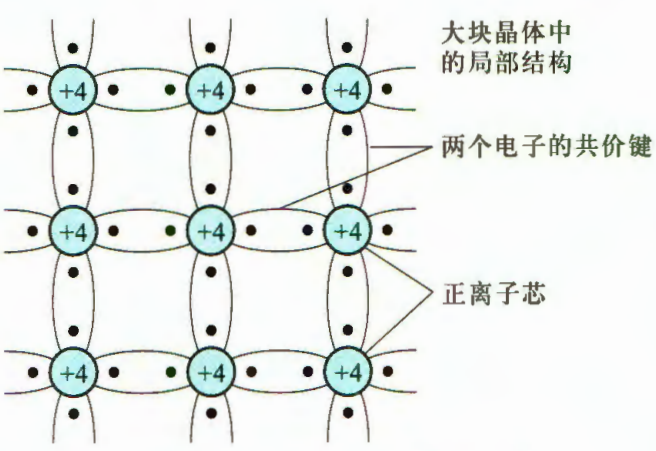
\includegraphics[width=0.4\textwidth]{pic/硅的二维结构.png}}\qquad
        \subcaptionbox{硅的三维结构示意图\cite{阎守胜}\label{硅的三维结构}}
        {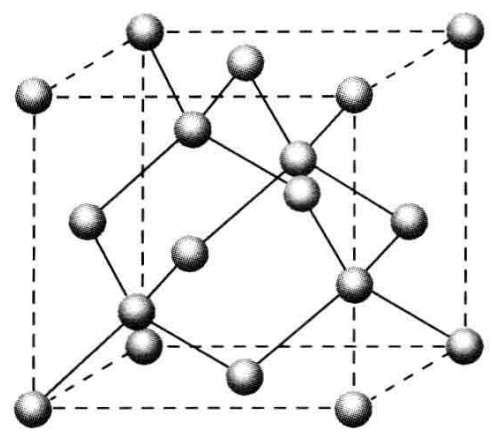
\includegraphics[width=0.3\textwidth]{pic/硅的三维结构.png}}
    \caption{硅的结构示意图\label{硅的结构示意图}}
\end{figure}

\subsubsection{二、本征激发}
半导体中能够自由移动的带电粒子称为\textbf{载流子}\index{Z!载流子};在室温下,部分价电子会挣脱共价键的束缚,成为\textbf{自由电子}\index{Z!自由电子},此时共价键中留下的空位称作\textbf{空穴}\index{K!空穴},这种现象称作\textbf{本征激发}\index{B!本征激发}。可以看到,本征半导体中有两种载流子——自由电子和空穴。当自由电子与空穴相遇就会填补空穴,这种现象称作\textbf{复合}\index{F!复合}。

总体上,温度越高,载流子浓度越大。因为温度越高热运动越剧烈,本征激发越多,随后复合的概率随之上升,最后本征激发和复合重新达到\textbf{动态平衡}。

\subsection{杂质半导体}
在室温下,本征激发产生的载流子浓度较低,且与温度密切相关,因此人们选择了掺杂来解决上述问题。

通过扩散工艺,在本征半导体中掺入少量杂质元素,就成为\textbf{杂质半导体}\index{Z!杂质半导体},如图\ref{P型半导体与N型半导体}所示。

若掺入五价元素(如磷),就成为\textbf{N型半导体}\index{N!N型半导体}(Negative),其中五价元素称为\textbf{施主杂质}\index{S!施主杂质},其中自由电子较多,称为\textbf{多子}\index{D!多子},而空穴较少,称为\textbf{少子}\index{S!少子}。若掺入三价元素(如硼),就成为\textbf{P型半导体}\index{P!P型半导体}(Positive),其中三价元素称为\textbf{受主杂质}\index{S!受主杂质}。

\begin{figure}[htb]
    \centering
    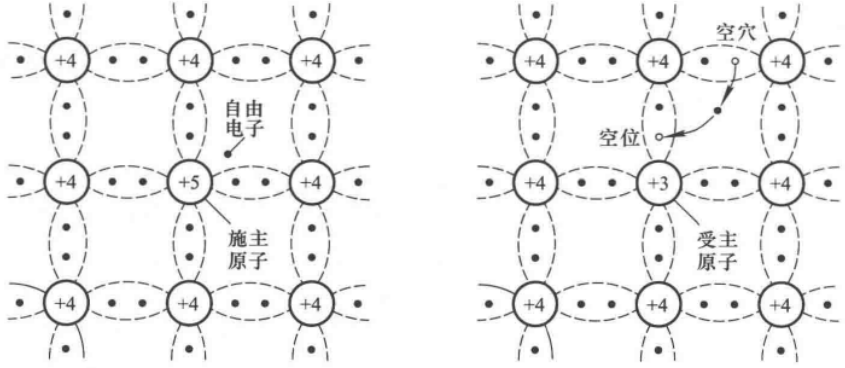
\includegraphics[width=0.8\linewidth]{pic/P型半导体与N型半导体.png}
    \caption{P型半导体与N型半导体\cite{华成英}\label{P型半导体与N型半导体}}
\end{figure}

注意,掺入P(磷)元素的本征半导体为N型半导体。

\subsection{PN结}
将P型半导体与N型半导体制作在同一块硅片上,在交界面处就形成了\textbf{PN结}\index{P!PN结}。\textbf{PN结具有单向导电性}。

\subsubsection{一、PN结的形成}
PN结的形成来源于\textbf{扩散运动}\index{K!扩散运动}和\textbf{漂移运动}\index{P!漂移运动}。其实漂移和扩散只不过是载流子运动的分解,分成了定向的运动和无规则的运动。

1.扩散运动:物质从浓度高的地方向浓度低的地方运动;

2.漂移运动:在电场的作用下载流子的运动。

\textbf{多子扩散}使得交界面处的电⼦和空⽳复合,形成\textbf{空间电荷区(PN结、耗尽区)}\index{K!空间电荷区}\index{H!耗尽区},进而此时内部形成由N区指向P区的内电场,促进\textbf{少子漂移},最终二者达到动态平衡。

当P区和N区杂质浓度不同时,称为\textbf{不对称PN结}\index{B!不对称PN结}。

\subsubsection{二、单向导电性}
1.外加正向电压时导通:

当P区电位高于N区电位时,称所加电压为\textbf{正向电压}\index{Z!正向电压},也称为\textbf{PN结正向偏置}。外加的正向电压削弱了内电场作用,使得少子漂移减少,多子扩散增加,耗尽层逐渐变窄。此时回路电流基本取决于扩散电流,称为正向电流$I_\mathrm{F}$,PN结表现为一个很小的电阻,也称为PN结正向导通。

2.外加反向电压时截止:

当N区电位高于P区电位时,称所加电压为\textbf{反向电压}\index{F!反向电压},也称为\textbf{PN结反向偏置}。此时耗尽区加宽,反向电流趋于0,但少子漂移运动增强,形成微弱的漂移电流,称为反向电流$I_\mathrm{R}$。

\subsubsection{三、PN结的伏安特性曲线}

\begin{figure}[htb]
    \centering
    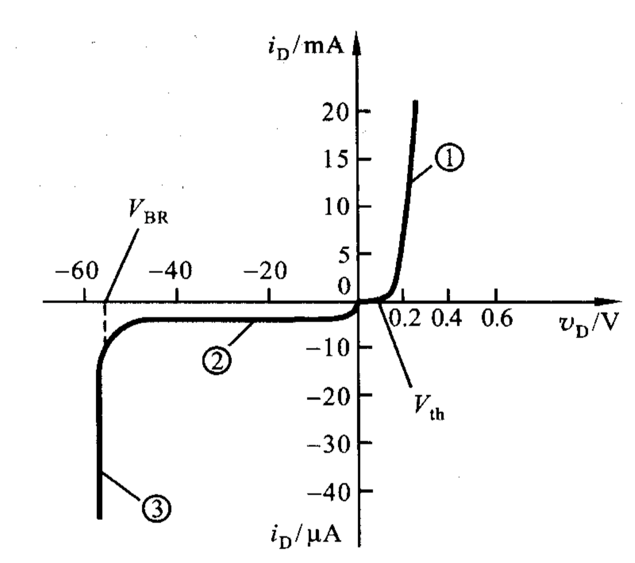
\includegraphics[width=0.5\linewidth]{pic/锗PN结的伏安特性曲线.png}
    \caption{PN结的伏安特性曲线(图片来源:曹平老师PPT-ch3)\label{PN结的伏安特性曲线}}
\end{figure}

不考虑击穿时,PN结两端的电压$v_\mathrm{D}$和电流$i_\mathrm{D}$的关系为

\begin{equation}
    i_{\mathrm{D}}=I_{\mathrm{S}}(\me^{\frac{v_\mathrm{D}}{nV_\mathrm{T}}}-1),
\end{equation}

通常,$n=1$,常温下\textbf{电压当量}\index{D!电压当量}$V_\mathrm{T}=\qty{26}{mV}$,$I_{\mathrm{S}}$为\textbf{反向饱和电流}\index{F!反向饱和电流}。

\textbf{PN结的伏安特性曲线,如图\ref{PN结的伏安特性曲线}所示。}

\subsubsection{四、PN结的反向击穿}
当反向电压大到一定数值时,反向电流突然增加,这种现象称为\textbf{反向击穿}。反向击穿电压记为$V_\mathrm{BR}$。PN结的击穿主要有以下两种原因:

1.\textbf{雪崩击穿}\index{X!雪崩击穿}(不可控):

掺杂浓度较低时,耗尽层较宽,高速少子将共价键中价电子撞出并形成电子-空穴对(\textbf{碰撞电离}),新的电子和空穴又撞出其他价电子,载流子雪崩式增加(\textbf{倍增效应});

2.\textbf{齐纳击穿}\index{Q!齐纳击穿}(可控——稳压二极管):

掺杂浓度较高时,耗尽层较窄,场强极大使得价电子直接从共价键中被拉出来,变成自由电子。

以上二者均可逆,但功率过高会发生不可逆的\textbf{热击穿}\index{R!热击穿}。

\subsubsection{五、PN结的电容特性}
一个器件的电压变化,储存的电荷量跟着变化,就会反映出电容特性。一般在高频丝滑才会考虑其电容特性。

1.\textbf{扩散电容}\index{K!扩散电容}:

穿过PN结未被复合的载流子称为\textbf{超量载流子}。在PN结附近,N区有空穴的积累,P区也有电子的积累,可以视为电荷存储到PN结邻域,外施电压的变化会导致PN结邻区存储电荷的变化,等效电容记作$C_\mathrm{D}$;

2.\textbf{势垒电容}\index{S!势垒电容}:

反偏时,离子在PN结交界处聚集形成的势垒区,是积累空间电荷的区域。电压改变时,引起空间电荷区大小变化,导致积累的空间电荷的改变,等效电容记作$C_\mathrm{B}$。

\section{二极管}
人们在发现PN结的特性后,将其包裹起来并引出两个电极,就形成了\textbf{二极管}\index{E!二极管}。
\subsection{二极管的结构}
二极管分为点接触型、面接触型、平面型。平面型二极管的结构示意图及二极管的代表符号如图\ref{二极管的结构及符号}所示。

\begin{figure}[htb]
    \centering
        \subcaptionbox{二极管的结构及符号\cite{康华光}\label{二极管的结构及符号}}
        {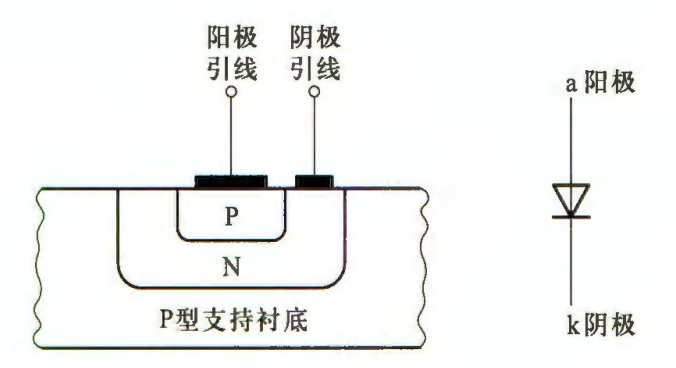
\includegraphics[width=0.4\textwidth]{pic/半导体二极管的结构及符号.png}}\qquad
        \subcaptionbox{齐纳二极管的符号\cite{康华光}\label{齐纳二极管的符号}}
        {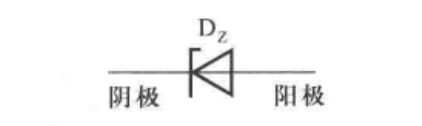
\includegraphics[width=0.3\textwidth]{pic/齐纳二极管的符号.png}}
        \caption{BJT的结构和符号\label{111}}
\end{figure}

齐纳二极管是一种面接触型晶体二极管,很容易形成强电场,符号如图\ref{齐纳二极管的符号}所示。齐纳二极管主要利用齐纳击穿在反向击穿特性$V_{\mathrm{Z}}$附近稳压,在电路中往往只会反接。

\subsection{二极管的伏安特性曲线及主要参数}

二极管的伏安特性和PN结的伏安特性基本相同。

\subsubsection{一、正向特性}

硅管的\textbf{门坎电压(死区电压)}\index{M!门坎槛电压}$V_{\mathrm{th}}$约为$\qty{0.5}{V}$;锗管的$V_{\mathrm{th}}$约为$\qty{0.1}{V}$。

\subsubsection{二、反向特性}
由于少数载流子的数目较少,所以反向电流很小,硅管的反向电流比锗管小得多。反向击穿特性则类似PN结。

\subsection{二极管基本电路及分析方法}
分析非线性电路的基本思想之一就是线性化,进而使用线性电路的分析方法。

\subsubsection{一、大信号模型}
1.\textbf{理想模型}:\index{L!理想模型}理想模型简单好用,但是比较粗糙,参考图\ref{二极管的三种等效模型}(a)。

2.\textbf{恒压降模型}:\index{H!恒压降模型}恒压降模型在⼆极管电路的分析中非常常用,参考图\ref{二极管的三种等效模型}(b)。硅管的正向导通压降约为$\qty{0.7}{V}$;锗管约为$\qty{0.2}{V}$(锗原子半径大,对外层电子束缚小,更易脱离共价键,导通电压低)。

3.\textbf{折线模型}:\index{Z!折线模型}折线模型考虑了动态电阻,但是略复杂,参考图\ref{二极管的三种等效模型}(c)。

\begin{figure}[htb]
    \centering
    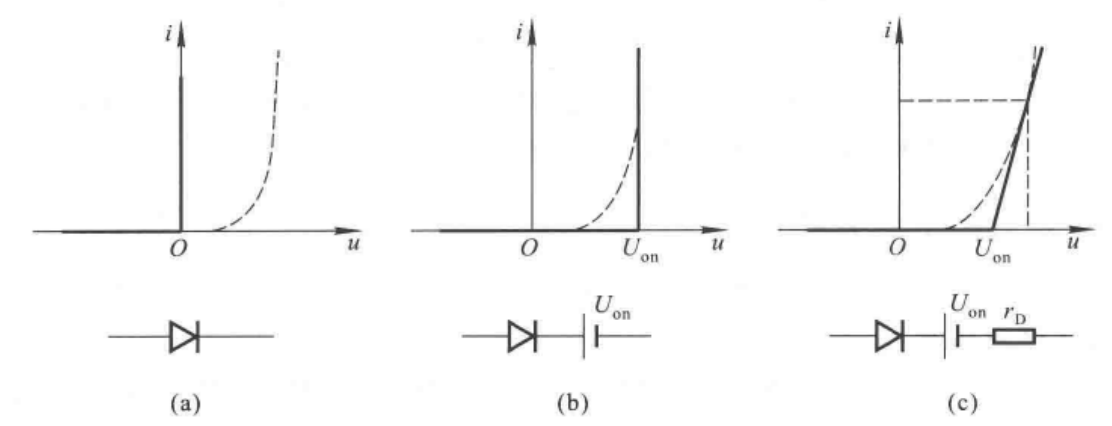
\includegraphics[width=0.8\linewidth]{pic/二极管的三种等效模型.png}
    \caption{二极管的三种等效模型\cite{华成英}\label{二极管的三种等效模型}}
\end{figure}

应用电路:整流电路、开关电路、限幅电路、钳位电路。注意模型和实际元件之间的区别。

二极管工作状态的分析:\textbf{假定全部二极管截止},然后计算每个二极管两端的电压是否大于导通电压。电压大的优先导通,然后再假设剩下的截止,重复上述分析,直到判定完所有二极管的工作状态。

\subsubsection{二、小信号模型}\index{X!小信号模型}
以上三个模型反映了二极管全部特性(除了反向击穿部分),可用于分析工作电压在较大范围内变化的情况,也称作\textbf{大信号模型}\index{D!大信号模型}。当仅仅考虑电压或者电流小幅波动时所建立的模型称为\textbf{小信号模型}。

\begin{figure}[htb]
    \centering
    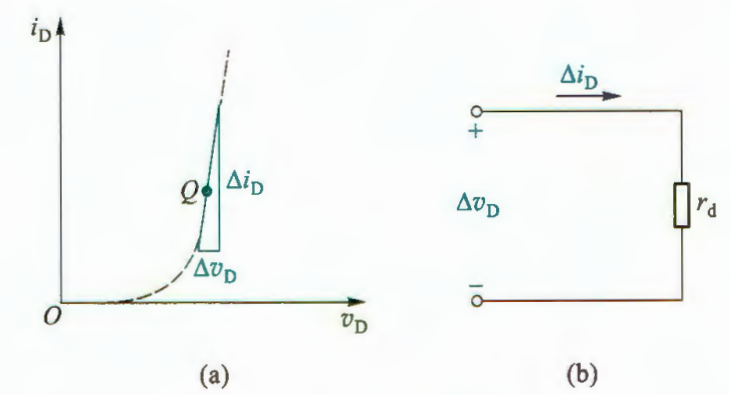
\includegraphics[width=0.6\linewidth]{pic/二极管的小信号模型.png}
    \caption{二极管的小信号模型\cite{康华光}\label{二极管的小信号模型}}
\end{figure}

小信号模型基本分析步骤将会在第二章详细讲解,此处仅做概述。

当电路中仅有直流信号时,称做\textbf{静态}\index{J!静态},$U-I$图上对应的点称作\textbf{静态工作点(Q点)}\index{J!静态工作点}。

二极管的小信号模型——\textbf{微变电阻}\index{W!微变电阻}$r_\mathrm{d}=\frac{V_\mathrm{T}}{I_\mathrm{D}}$,其中$V_\mathrm{T}$为电压当量,$I_\mathrm{D}$为Q点电流。

\section{双极结型三极管(BJT)}\index{S!双极结型三极管}
将两个二极管背靠背拼接起来,就成为了一个三极管。三极管分主要为双极结型三极管(BJT)和场效应三极管(FET)两种。虽然如今广泛应用的三极管主要是MOSFET,但BJT在个别领域也有其优势。由于本课程更侧重于BJT的使用,因此首先讲解BJT。

\textbf{双极结型晶体管(Bipolar Junction Transistor, BJT)}\index{S!双极结型晶体管},又称为半导体三极管或晶体管。其中\textbf{双极型器件}\index{S!双极型器件}是指由电子和空穴两种载流子都参与导电的半导体器件。

\subsection{结构及类型}
\subsubsection{一、结构:三个区域、三个电极、两个PN结}
BJT的结构如图\ref{集成电路中典型NPN型BJT的截面图}所示,可以看到三个区域的一些基本特点:

1.\textbf{发射区/发射极}\index{F!发射区}\index{F!发射极}e(emitter):需要发射载流子,因此掺杂浓度最高,和基区形成\textbf{发射结};

2.\textbf{集电区/集电极}\index{J!集电区}\index{J!集电极}c(collector):需要收集载流子,因此面积最大且掺杂浓度较低,和基区形成\textbf{集电结};

3.\textbf{基区/基极}\index{J!基区}\index{J!基极}b(base):很薄且杂质浓度低,起到控制作用。

\begin{figure}[htb]
    \centering
        \subcaptionbox{集成电路中典型NPN型BJT的截面图\cite{康华光}\label{集成电路中典型NPN型BJT的截面图}}
        {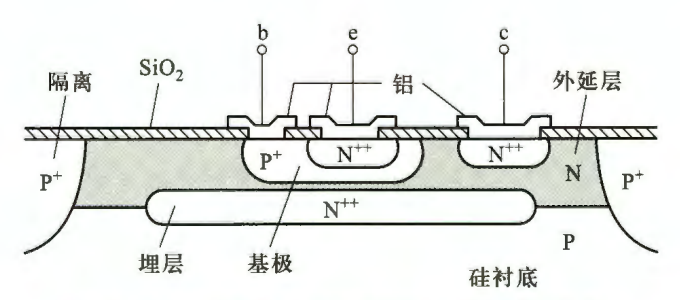
\includegraphics[width=0.68\textwidth]{pic/集成电路中典型NPN型BJT的截面图.png}}\qquad
        \subcaptionbox{BJT的符号\cite{华成英}\label{BJT的符号}}
        {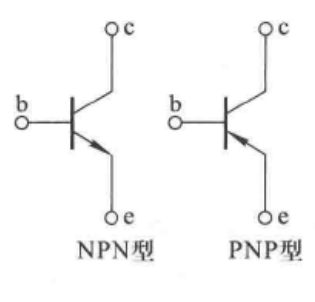
\includegraphics[width=0.28\textwidth]{pic/BJT的符号.png}}
        \caption{BJT的结构和符号\label{BJT的结构和符号}}
\end{figure}

\subsubsection{二、类型}
BJT分为PNP型和NPN型,如图\ref{BJT的符号}所示。注意箭头在基极b和发射极e之间,方向为P指向N。

除非特殊声明,本手册之后所有的BJT均考虑为NPN型。

\subsection{BJT的电流放大作用}
放大是对模拟信号最基本的处理,而三极管是放大电路的核心,它能够控制能量的转换,使微小信号不失真地放大输出。本手册第二章将会专门讨论放大相关的内容。

BJT的放大作用主要体现体现在小的基极电流可以控制大的集电极电流——\textbf{电流控制电流源}。

\subsubsection{一、内部载流子的运动}
\begin{figure}[htb]
	\centering
	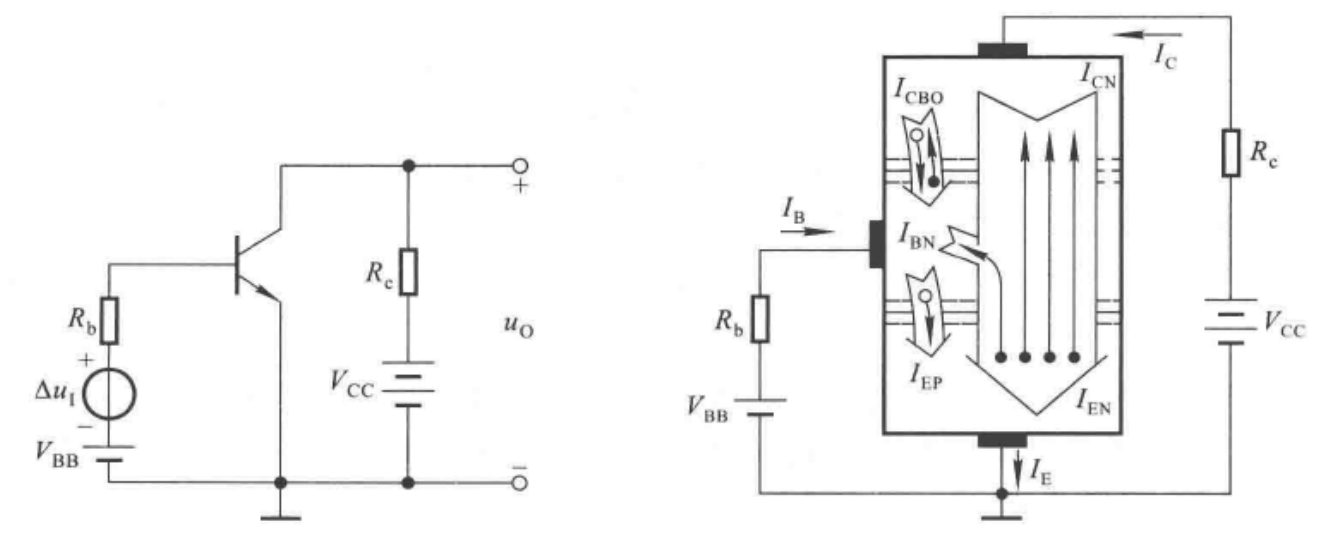
\includegraphics[width=0.8\linewidth]{pic/BJT原理.png}
	\caption{BJT放大的基本原理\cite{华成英}\label{BJT放大}}
\end{figure}

1.发射结正偏:发射区有大量自由电子向基区\underline{扩散},同时基区有少量空穴向发射区\underline{扩散},形成$I_{\mathrm{EN}}$和$I_{\mathrm{EP}}$。由于两个区域掺杂浓度不同,$I_{\mathrm{EN}}\gg I_{\mathrm{EP}}$。扩散运动形成发射极电流$I_{\mathrm{E}}$。

2.基区:由于基区薄且掺杂浓度低,扩散到基区的电子只有极少部分与空穴复合,其余均到达集电极。由于外部电源$V_{\mathrm{BB}}$的存在,自由电子被不断抽走,使得基区空穴浓度保持不变,因此发射区扩散到基区的电子和基区空穴源源不断地复合。这样不断地复合和产生,宏观上形成基极电流$I_{\mathrm{B}}$,而向集电结\underline{漂移}的电子形成$I_{\mathrm{CN}}$。

注意,BJT工作在放大状态的时候,复合的比例是固定的,因此有了“放大倍数”的概念。

3.集电结反偏:由于集电结面积大且反向偏置,它尽可能地在收集从发射区过来的电子,保证从发射区到基区浓度梯度的稳定。当反向偏置到达一定程度后,收集电子能力和偏置电压无关。

\subsubsection{二、常用参数}
由基尔霍夫电流定律可以得到$I_{\mathrm{E}}=I_{\mathrm{B}}+I_{\mathrm{C}}$,其他参数如下:

1.(共射直流)放大系数\index{F!(BJT)(共射直流)放大系数}:
\begin{equation}
    \bar{\beta}=\frac{I_{\mathrm{CN}}}{I_{\mathrm{BN}}}\approx\frac{I_{\mathrm{C}}}{I_{\mathrm{B}}}.
\end{equation}

2.(共基直流)放大系数\index{F!(BJT)(共基直流)放大系数}:
\begin{equation}
    \bar{\alpha}=\frac{I_{\mathrm{CN}}}{I_{\mathrm{E}}}\approx\frac{I_{\mathrm{C}}}{I_{\mathrm{E}}}=\frac{\bar{\beta}}{1+\bar{\beta}}.
\end{equation}

3.(共射交流)放大系数$\beta$、(共基交流)放大系数$\alpha$。

除非特殊声明,一般认为$\beta=\bar{\beta}$和$\alpha=\bar{\alpha}$。

\subsection{BJT共射特性曲线}
之前总是讨论⼆端元件的伏安特性。⼆端元件只有⼀个电流和电压的概念。但是BJT是⼀个三端元件,因此需要⽤多个关系来刻画其伏安特性。BJT放大信号时,主要有三种连接方式:共基、共射、共集。这里仅简单介绍共射特性曲线。

\subsubsection{一、输入特性曲线:}
输入特性曲线用函数关系表示为:
\begin{equation}
    i_\mathrm{B}=f(v_{\mathrm{BE}})|_{v_{\mathrm{CE}}=\mathrm{Const.}}
\end{equation}

\begin{figure}[htb]
    \centering
    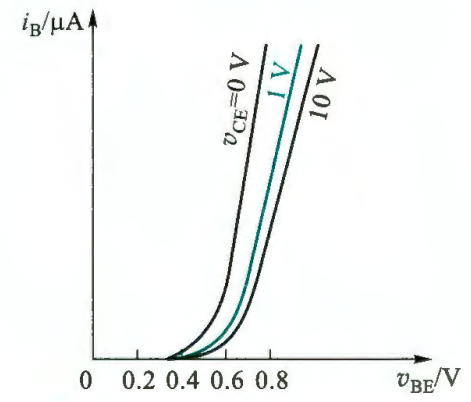
\includegraphics[width=0.35\linewidth]{pic/BJT共射输入特性曲线.png}
    \caption{BJT共射输入特性曲线\cite{康华光}\label{BJT共射输入特性曲线}}
\end{figure}

输入特性曲线如图\ref{BJT共射输入特性曲线}所示。当$v_{\mathrm{CE}}=\qty{0}{V}$时,发射结与集电结并联。

发射结正偏时,输入特性曲线就是PN结正向的伏安特性曲线。同样的$v_{\mathrm{BE}}$下,随着$v_{\mathrm{CE}}$增加,集电极收集载流子能力增加,使得载流子在基区停留时间较短,从而$i_\mathrm{B}$减小,这意味着同样的$v_{\mathrm{BE}}$下$i_\mathrm{B}$更小。

当$v_{\mathrm{CE}}=\qty{1}{V}$时,发射的电子几乎都被集电区收集,电流几乎不再减小。

\subsubsection{二、输出特性曲线:}
输出特性曲线用函数关系表示为:
\begin{equation}
    i_\mathrm{C}=f(v_{\mathrm{CE}})|_{i_{\mathrm{B}}=\mathrm{Const.}}
\end{equation}

\begin{figure}[htb]
    \centering
    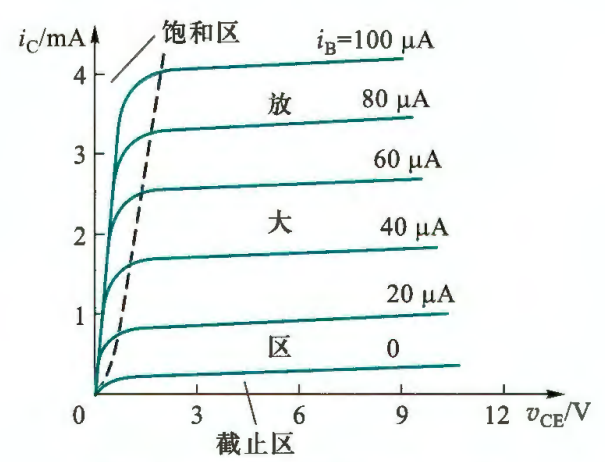
\includegraphics[width=0.45\linewidth]{pic/BJT共射输出特性曲线.png}
    \caption{BJT共射输出特性曲线\cite{康华光}\label{BJT共射输出特性曲线}}
\end{figure}

输出特性曲线的图比输入特性曲线更重要,如图\ref{BJT共射输出特性曲线}所示。可以看出,输出特性曲线分为三个部分:放大区、饱和区和截止区。在模电里,大部分时候BJT只会工作在放大区当放大器件,而在数电里会使BJT工作在饱和区和截止区当开关器件。

当$v_{\mathrm{CE}}=\qty{0}{V}$时,集电结正偏,不能收集载流子,因此$i_{\mathrm{C}}=0$。

1.\textbf{放大区}\index{F!放大区}:工作条件为发射结正偏$v_{\mathrm{BE}}>V_{\mathrm{th}}$、集电结反偏。此时$i_{\mathrm{C}}$受到$i_{\mathrm{B}}$控制,有$i_{\mathrm{C}}=\beta i_{\mathrm{B}}$。

2.\textbf{饱和区}\index{B!(BJT)饱和区}:工作条件为发射结正偏、集电结正偏。此时$v_{\mathrm{CE}}$很小,载流子收集能力较弱。$i_{\mathrm{C}}$几乎不依赖于$i_{\mathrm{B}}$,其中的倾斜主要是因为基区宽度调制效应。此时有$i_{\mathrm{C}}<\beta i_{\mathrm{B}}$。

3.\textbf{截止区}\index{J!截止区}:工作条件为发射结反偏、集电结反偏(准确来说是发射结电压小于开启电压)。BJT无法导通,因此$i_{\mathrm{B}}=0,i_{\mathrm{C}}=I_{\mathrm{CEO}}$。

\section{场效应管(FET)}\index{C!场效应管}
\textbf{场效应管(Field Effect Transistor, FET)},顾名思义,就是利用电场的效应来控制输出电流的一种器件。对于FET,掌握其中的基本概念即可。

FET主要分为两类,结型场效应管\index{C!场效应管!结型场效应管(JFET)}和金属-氧化物-半导体场效应管。与三极管相比,在输出回路输出相同的电流,需要的输入电流的代价更小;同时,因为少子不参与导电,场效应管温度稳定性高,也因此属于\textbf{单极型器件}\index{D!单极型器件}。

\subsection{金属-氧化物-半导体场效应管(MOSFET)}
\textbf{金属-氧化物-半导体场效应管(Metal-Oxide-Semiconductor FET)}\index{C!场效应管!金属-氧化物-半导体场效应管(MOS管)},又称为\textbf{绝缘栅型场效应管}\index{J!绝缘栅型场效应管},或简称为MOS管,目前在大规模集成电路中占据了主导地位。

从载流子的类型来看,分为N沟道MOSFET和P沟道MOSFET;从沟道形成机理来分又各自分为增强型E型(Enhancement)和耗尽型D型(Depletion),将二者两两组合,就形成了四种不同的MOS管。

本节主要讲N沟道增强型MOSFET。

\subsubsection{一、结构}
在低掺杂的P型半导体衬底上生长两个高掺杂的N区,就形成了两个背靠背的PN结,再在衬底上生长一层二氧化硅,并安装三个铝电极,就形成了N沟道增强型MOS管。由制作工艺可以看到其由金属铝、氧化物二氧化硅和半导体硅构成,MOS管也因此得名。

N沟道增强型MOSFET的结构如图\ref{N沟道增强型MOSFET结构}所示,三个区域分别有一些基本特点:

1.\textbf{栅极}\index{S!栅极}g(gate):类比BJT基极b。由于栅极下面有绝缘层二氧化硅,源极、栅极与漏极之间无电接触,有着很高的输入电阻,因此称为“绝缘栅型”场效应管。

2.\textbf{源极}\index{Y!源极}s(source):类比BJT发射极e,提供载流子。

3.\textbf{漏极}\index{L!漏极}d(drain):类比BJT集电极c,载流子流出。一般而言,漏极d与源极s是对称的。但人们往往会将源极s和衬底连接在一起使用,这样栅极和衬底各相当于一个极板,形成电容。当栅-源电压变化时就能改变绝缘层中的感应电荷的多少,从而控制漏极电流。

如图\ref{N沟道增强型MOSFET符号},增强型MOSFET中间为短划线,这意味着$v_{\mathrm{GS}}=0$时沟道断开,而其中箭头指向PN结导通的方向。

\begin{figure}[htb]
    \centering
        \subcaptionbox{N沟道增强型MOSFET结构\cite{康华光}\label{N沟道增强型MOSFET结构}}
        {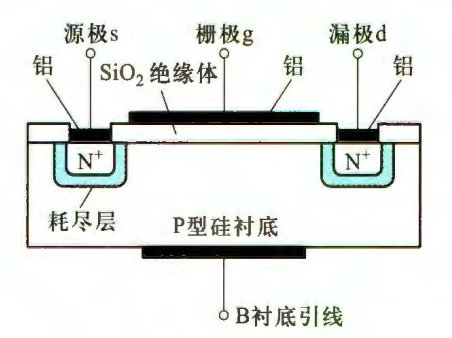
\includegraphics[width=0.45\textwidth]{pic/N沟道增强型MOSFET结构.png}}\qquad
        \subcaptionbox{增强型MOSFET符号\cite{华成英}\label{N沟道增强型MOSFET符号}}
        {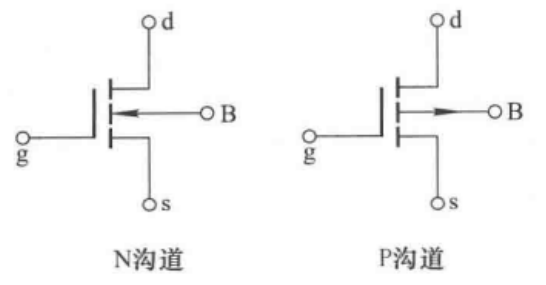
\includegraphics[width=0.45\textwidth]{pic/N沟道增强型MOSFET符号.png}}
        \caption{增强型MOSFET的结构和符号\label{N沟道增强型MOSFET}}
\end{figure}

\subsubsection{二、工作原理}
1.$v_{\mathrm{GS}}=0$,没有\textbf{导电沟道}\index{D!导电沟道},如图\ref{N沟道增强型MOSFET的基本工作原理}(a)所示。即使漏极和源极之间有电压也不会有电流,也因此称为增强型FET。

2.$v_{\mathrm{GS}}\geq V_{\mathrm{TN}}$,出现N型沟道,如图\ref{N沟道增强型MOSFET的基本工作原理}(b)所示。由于绝缘层的存在,不会产生栅极电流,但是会产生指向衬底的强电场,排斥P型衬底中的多子空穴,同时吸引少子自由电子。当$v_{\mathrm{GS}}$大于\textbf{阈值电压}\index{Y!阈值电压}$V_{\mathrm{TN}}$,绝缘层下方形成\textbf{反型层(导电沟道、感生沟道)}\index{F!反型层}。此时N沟道类似于一个被电压控制的可变电阻器,$v_{\mathrm{GS}}$越大,沟道越宽,ds之间的电阻越小。

\begin{figure}[htb]
    \centering
    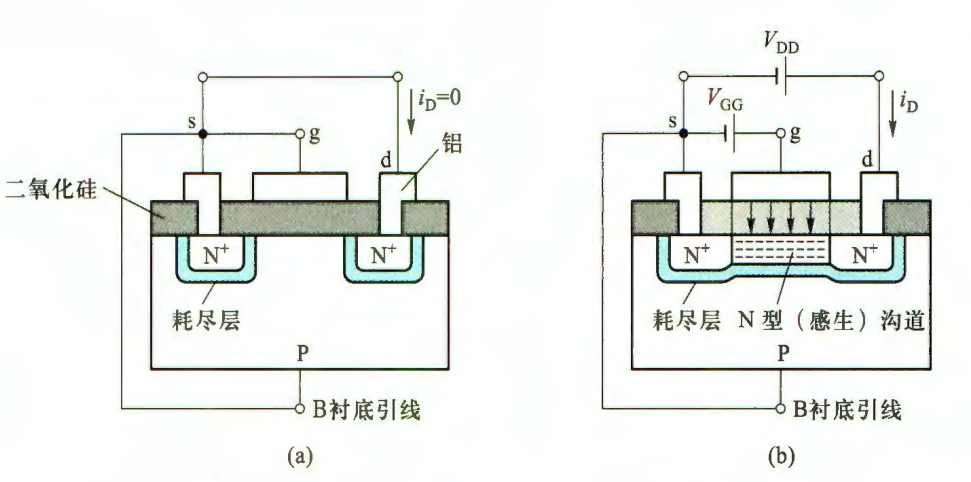
\includegraphics[width=0.65\linewidth]{pic/N沟道增强型MOSFET的基本工作原理.png}
    \caption{N沟道增强型MOSFET的基本工作原理\cite{康华光}\label{N沟道增强型MOSFET的基本工作原理}}
\end{figure}

3.感生沟道出现后,保持$v_{\mathrm{GS}}$不变,施加正的$v_{\mathrm{DS}}$,产生漏极电流$i_{\mathrm{D}}$,同时沟道厚度从左至右不断变薄,如图\ref{可变电阻区和恒流区的形成机制}(a)所示。当$v_{\mathrm{DS}}$较小时,$i_{\mathrm{D}}$与$v_{\mathrm{DS}}$近似线性,此时可等效为\textbf{沟道电阻}\index{G!沟道电阻}。由于$v_{\mathrm{GS}}$可控制沟道电阻大小,因此被称为\textbf{可变电阻区}\index{K!可变电阻区}。

当$v_{\mathrm{DS}}$增大到$v_{\mathrm{DS}}=v_{\mathrm{GS}}-V_{\mathrm{TN}}$时,沟道的漏极侧会被夹断,称为\textbf{预夹断}\index{Y!预夹断},如图\ref{可变电阻区和恒流区的形成机制}(b)所示。若$v_{\mathrm{DS}}$继续增大,由于夹断区电阻远大于沟道其余部分电阻,增加的电压都会落到夹断区,导致其余部分的电压几乎不增加,$i_\mathrm{D}$几乎不随$v_{\mathrm{DS}}$改变,称为\textbf{恒流区}\index{H!恒流区}。

\begin{figure}[htb]
    \centering
    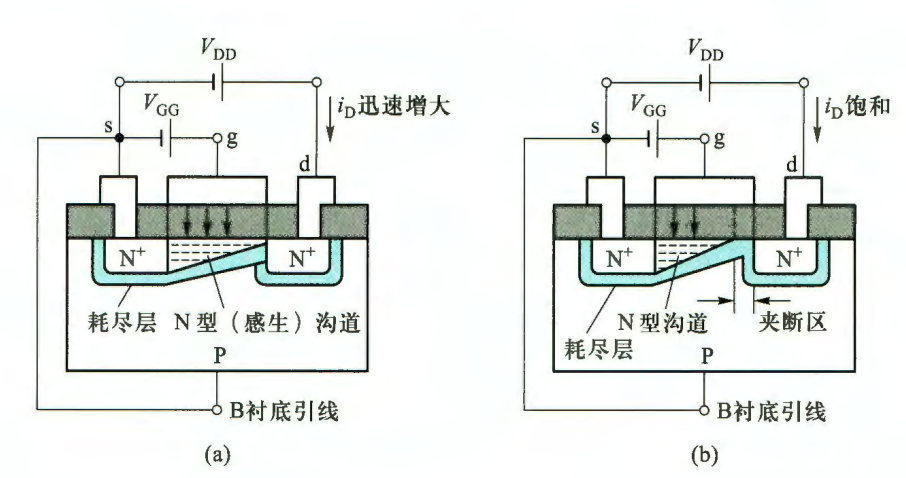
\includegraphics[width=0.65\linewidth]{pic/可变电阻区和恒流区的形成机制.png}
    \caption{可变电阻区和恒流区的形成机制\cite{康华光}\label{可变电阻区和恒流区的形成机制}}
\end{figure}

这样,就得到了一个\textbf{电压控制电流源}——由电压$v_{\mathrm{GS}}$控制的电流$i_\mathrm{D}$。

\subsubsection{三、N沟道耗尽型MOSFET}
\begin{figure}[htb]
    \centering
    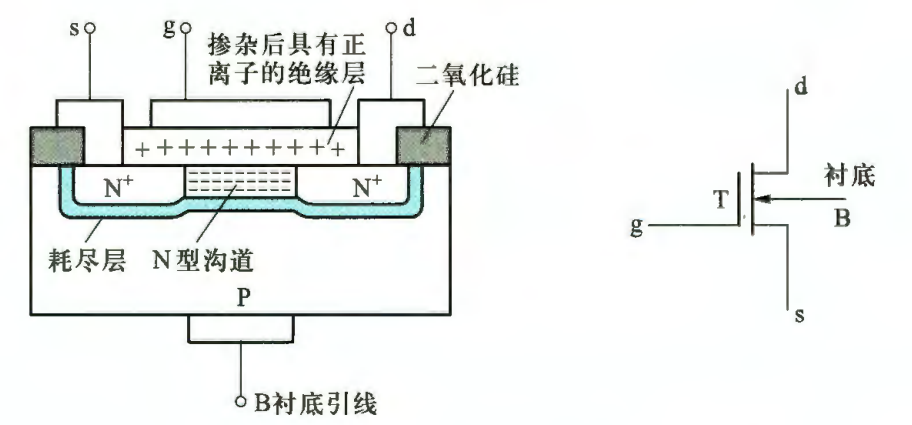
\includegraphics[width=0.6\linewidth]{pic/N沟道耗尽型MOSFET结构和符号.png}
    \caption{N沟道耗尽型MOSFET结构和符号\cite{康华光}\label{N沟道耗尽型MOSFET结构和符号}}
\end{figure}

与增强型不同的是,N沟道耗尽型MOSFET中在二氧化硅绝缘层中加入了大量的正离子(相当于人为先制造一个电场),那么即使$v_{\mathrm{GS}}=0$,也会形成反型层沟道。如图\ref{N沟道耗尽型MOSFET结构和符号}所示,从元件符号来看,ds之间是联通的。

当且仅当$v_{\mathrm{GS}}$为负且达到某一值时,反型层会消失,这个临界值称为\textbf{夹断电压}\index{J!夹断电压}$V_{\mathrm{TN}}$。其余规律和N沟道增强型MOSFET相同。

\subsection{N沟道增强型MOSFET特性曲线}
\subsubsection{一、输出特性曲线}
输出特性曲线的函数关系表示为:
\begin{equation}
    i_\mathrm{D}=f(v_{\mathrm{DS}})|_{v_{\mathrm{GS}}=\mathrm{Const.}}
\end{equation}

\begin{figure}[htb]
    \centering
    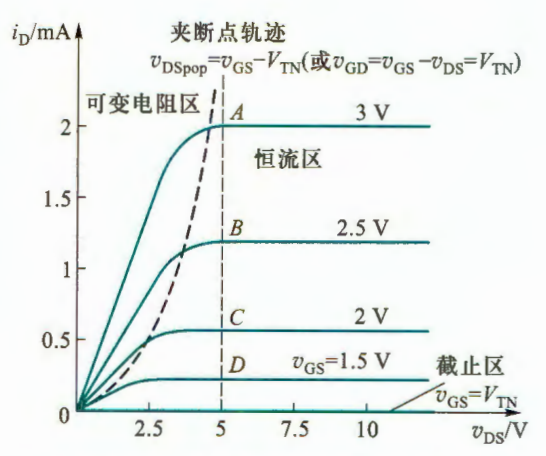
\includegraphics[width=0.45\linewidth]{pic/增强型NMOS管输出特性.png}
    \caption{增强型NMOS管输出特性\cite{康华光}\label{增强型NMOS管输出特性}}
\end{figure}

增强型NMOS管输出特性曲线如图\ref{增强型NMOS管输出特性}所示,与BJT类似,同样可以分为三个区:

1.\textbf{截止区}\index{J!截止区}:当$v_{\mathrm{GS}}<V_{\mathrm{TN}}$时,导电沟道尚未形成,$i_\mathrm{D}=0$。

2.\textbf{可变电阻区}\index{K!可变电阻区}。

3.\textbf{恒流区(放大区)}\index{H!恒流区}。

\subsubsection{二、转移特性}
FET是电压控制器件,由于栅极输入端基本没有电流,故讨论它的输入特性是没有意义的。因此考虑其转移特性曲线,函数关系表示为:

\begin{equation}
    i_\mathrm{D}=f(v_{\mathrm{GS}})|_{v_{\mathrm{DS}}=\mathrm{Const.}}
\end{equation}

\begin{figure}[htb]
    \centering
    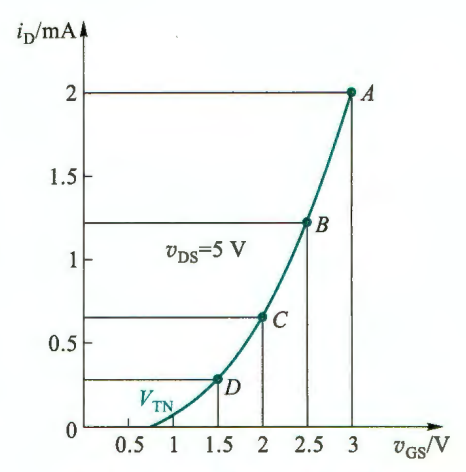
\includegraphics[width=0.35\linewidth]{pic/增强型NMOS管的恒流区转移特性.png}
    \caption{增强型NMOS管的恒流区转移特性\cite{康华光}\label{增强型NMOS管的恒流区转移特性}}
\end{figure}

增强型NMOS管转移特性曲线如图\ref{增强型NMOS管的恒流区转移特性}所示,是一条二次曲线。注意,当工作在恒流区时,才能给出图\ref{增强型NMOS管的恒流区转移特性}。如果是耗尽型,那么只需要将$v_{\mathrm{GS}}$出现的地方做⼀个平移,其他保持不变即可。如果是P沟道,只需要将坐标反向(图像反转180度)。

\subsection{结型场效应管(JFET)}
\textit{(本节的内容仅做了解)}

\textbf{结型场效应管(Junction FET)}\index{C!场效应管!结型场效应管(JFET)}也分为P沟道和N沟道两种类型。由于JFET具体原理与MOS管大同小异,因此不详细展开,本节简单仅讨论N沟道JFET。

\subsubsection{一、结构}
如图\ref{N沟道JFET结构示意图}所示,在同一块N型半导体上制作两个高掺杂的P区,并连接在一起,形成栅极g。N型半导体两端引出两个电极为源极s和漏极d,漏极和源极之间的非耗尽层称为\textbf{导电通道}。

\begin{figure}[htb]
    \centering
    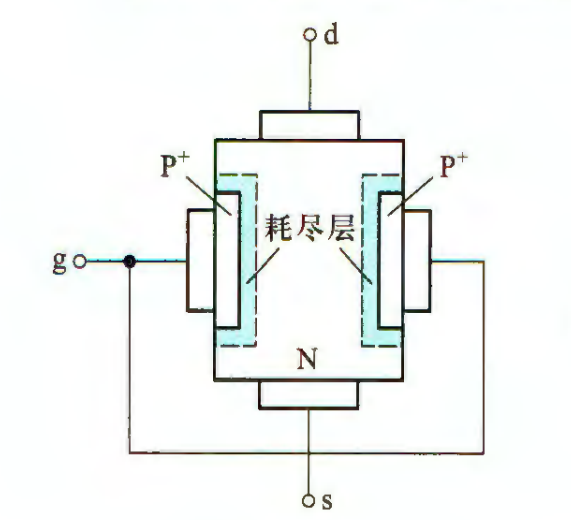
\includegraphics[width=0.35\linewidth]{pic/N沟道JFET结构示意图.png}
    \caption{N沟道JFET结构示意图\cite{康华光}\label{N沟道JFET结构示意图}}
\end{figure}

\subsubsection{二、工作原理}
首先,对于N沟道结型场效应管,当$v_{\mathrm{GS}}>0$时,PN结导通,此时$v_{\mathrm{GS}}$不能实现对沟道电流的控制,因此以下$v_{\mathrm{GS}}$增大全部指的是绝对值增大。

1.$v_{\mathrm{DS}}$,$v_{\mathrm{GS}}$增大时,耗尽层加宽,沟道变窄,沟道电阻增大。当增大到\textbf{夹断电压}$V_\mathrm{P}$时,沟道全部被夹断,沟道电阻变为无穷大。

2.当$V_\mathrm{P}<v_{\mathrm{GS}}<0$时,$v_{\mathrm{DS}}$较小时,由于$v_{\mathrm{GD}}$逐渐减小,靠近漏极的导电沟道逐渐变窄,随后预夹断。此时若$v_{\mathrm{DS}}$继续增大,则耗尽层闭合部分沿着沟道延伸,此时$v_{\mathrm{DS}}$的增大几乎全部用于克服夹断区延伸产生的电阻上,此时$i_\mathrm{D}$恒流。

3.当$v_{\mathrm{DS}}$继续增大时,可能会发生耗尽区击穿(二极管的反向击穿)。
    \chapter{基本放大电路}
绪论中提到了模拟电路就是用来处理生活中各种模拟信号,以满足人们的需要。生活中的信号通常是很微弱的,一般情况下都难以直接显示或者处理,这时候就需要放大电路。

在上一章中已经介绍了一些基本的元件及其特性,而本章将利用这些元件组成基本放大电路,并提出一套分析放大电路的方法。

\section{放大电路的基本构成}

\subsection{放大的概念}
在不同领域中都存在放大的概念,而在模拟电路中的放大都是指对于\textbf{变化量}的放大。这些变化的信号往往都可以由傅里叶分解为若干正弦信号的叠加,因此在模电中常常讨论的是对于\textbf{正弦交流信号}的放大。

教室中,老师的声音可以通过扬声器放大,而实际上是麦克风处的输入功率经过放大后,通过扬声器的输出。由此可以看出,放大的基本特征是对功率的放大,是在对能量进行控制和转换。而为了能够控制能量,电路中应当存在相应控制能量的元件,即\textbf{有源元件}\index{Y!有源元件}(例如晶体管、场效应管)。由能量守恒可以知道,多出来的功率并不是凭空产生的,也不会来源于电路中的有源元件,而是从电路中的直流电源中获得的。

此外,如果扬声器发出的声音失真则毫无意义,因此放大电路的一个基本要求就是不失真。通常说的放大均为\textbf{线性放大},也就是在信号整体上做⼀个倍乘,而波形保持原来的形状不变。输出波形的变形称为\textbf{失真}\index{S!失真}。

\subsection{放大电路的性能指标}\label{放大电路的性能指标}
为了衡量不同放大电路的各方面性能,人们提出了多种指标。而对于本课程,主要围绕放大倍数、输入电阻和输出电阻三个指标分析放大电路。

\subsubsection{一、放大倍数}
\textbf{放大倍数}\index{F!放大倍数}用于衡量电路放大能力。由输出和输入参数的不同,可以定义四个放大倍数,即\textbf{电压增益}\index{F!放大倍数!电压增益}$A_v=v_\mathrm{o}/v_\mathrm{i}$,\textbf{电流增益}\index{F!放大倍数!电流增益}$A_i=i_\mathrm{o}/i_\mathrm{i}$,\textbf{互阻增益}\index{F!放大倍数!互阻增益}$A_r=v_\mathrm{o}/i_\mathrm{i}$,\textbf{互导增益}\index{F!放大倍数!互导增益}$A_g=i_\mathrm{o}/v_\mathrm{i}$。其中A表示Amplification,A的下标$v,i,r,g$表示电压、电流、电阻、电导。

对于无量纲的电压增益和电流增益,一般会用\textbf{对数增益}表示,$\text{增益}=20\log|A|\,\si{dB}$。注意,这里底数是10。比如强度衰减到原来的$1/10$,就说增益是$\qty{-20}{dB}$,而$\qty{-3}{dB}$就是衰减到原来的⼀半。$\text{功率增益}=10\log|A_p|\,\si{dB}$。

\subsubsection{二、输入电阻}
\textbf{输入电阻}\index{S!输入电阻}反映放大电路索取信号源的大小,定义为$R_\mathrm{i}=v_\mathrm{i}/i_\mathrm{i}$,其中下标i表示input。定量分析时,一般会选择外加测试电压$v_\mathrm{t}$,并产生相应的测试电流$i_\mathrm{t}$,$R_\mathrm{i}=v_\mathrm{t}/i_\mathrm{t}$。

注意输入电阻中不会出现信号源内阻$R_{\mathrm{i}}$。

\subsubsection{三、输出电阻}
\textbf{输出电阻}\index{S!输出电阻}反映放大电路带负载的能力,定义为$R_\mathrm{o}=v_\mathrm{o}/i_\mathrm{o}|_{v_\mathrm{s}=0,R_\mathrm{L}=\infty}$,其中下标o(建议不要写成0)表示output。定量分析时,要先将信号源$v_\mathrm{s}=0$置零,负载$R_\mathrm{L}$开路。

注意输出电阻中不会负载$R_{\mathrm{L}}$。

\begin{figure}[htb]
    \centering
    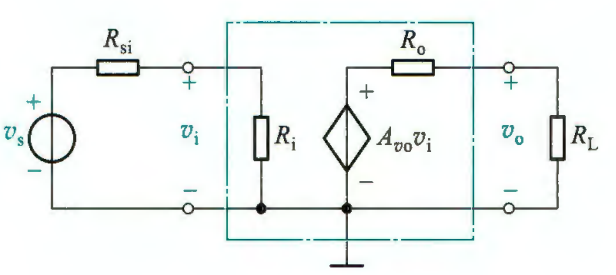
\includegraphics[width=0.5\linewidth]{pic/电压放大电路模型.png}
    \caption{电压放大电路模型\cite{康华光}\label{电压放大电路模型}}
\end{figure}

举一个简单的例子。图\ref{电压放大电路模型}为电压放大电路,其中$R_\mathrm{i}$为输入电阻,$R_\mathrm{o}$为输出电阻,则实际电压增益为
\begin{equation}
    A_v=A_{v\mathrm{o}}\frac{R_{\mathrm{L}}}{R_{\mathrm{L}}+R_{\mathrm{o}}}
\end{equation}

⼀个类似概念是\textbf{源放大倍数}:
\begin{equation}
    A_{v\mathrm{s}}=\frac{v_{\mathrm{o}}}{v_{\mathrm{s}}}=\frac{v_{\mathrm{o}}}{v_{\mathrm{i}}}\cdot \frac{v_{\mathrm{i}}}{v_{\mathrm{s}}}=A_v\frac{R_{\mathrm{i}}}{R_{\mathrm{si}}+R_{\mathrm{i}}}.
\end{equation}

由上面两个公式可知,当$R_\mathrm{i}=0,R_\mathrm{o}=\infty$时,可以避免负载电路对增益的影响以及信号在信号源上的衰减。因此,电压放大电路适用于信号源内阻较小而负载较大的情况,对其他三种类型的电路也可以进行类似的分析。

\section{放大电路的分析方法}
所谓的分析放大电路,本质上是去求解一个复杂的时变非线性方程(组),但这个方程(组)基本无法严格求解。在实际应用中,往往没有精确计算的必要,只要在设计误差范围内可以使用就行了。因此,人们提出了\textbf{图解法}\index{T!图解法}和\textbf{小信号模型法}\index{X!小信号模型法}来近似求解电路。两种方法在本质上都充分利用了“小信号”足够小的特点,类似于泰勒展开保留到一阶项,使得电路线性化,从而可以充分利用线性电路的分析方法。

在介绍这两种方法之前,先讲解一下放大电路通常进行的分解。

\subsection{直流通路和交流通路}
由放大电路的工作原理,放大电路中往往是直流量和交流量共存。其中直流分量往往用于提供工作点,使得三极管能够起到放大信号的作用,而交流分量才是真正被放大的部分。

此外,由于电路中有电容和电感的存在,直流量和交流量的流经的通路不同,因此需要引入直流通路和交流通路。这种思想类似于叠加定理,但值得注意的是,叠加定理仅对于线性电路成立,而此处的三极管为非线性元件。后面会看到,对于同样一个信号,由于放大电路的静态工作点不同,其对交流信号的放大倍数也不同,必须先求解静态工作点然后再做交流等效,这也能说明分解为直流通路和交流通路并非简单的叠加定理。

\subsubsection{一、直流通路}
\textbf{静态}\index{J!静态}是在放大电路没有输入信号时,电路中各处电压、电流都是不变的情况。而\textbf{直流通路}\index{Z!直流通路}是在直流电源作用下,直流电流流经的通路,用于对静态工作点的估算和对有源元件工作状态的判定。

对于直流通路,需要将电容视为开路,交流电源置零。

\subsubsection{二、交流通路}
\textbf{动态}\index{D!动态}是在放大电路存在输入信号后,电路中各处电压、电流都处于动态工作的情况。\textbf{交流通路}\index{J!交流通路}是交流输入信号下交流信号流经的通路,用于研究动态参数。

对于交流通路,需要将电容视为短路,直流电源置零(即电压源短路,电流源开路)。

\subsection{图解法}
图解法往往简单直观地反映了晶体管工作情况,但是必须实测所用管的特性曲线,且进行定量分析时误差较大。由于图解法有助于理解为什么说动态是建立在静态的基础上的,因此在此简单介绍。

\subsubsection{一、静态工作点的确定}
在输入回路中,Q点应当既在输入特性曲线上,又应满足外电路的回路方程。对于输出回路也类似。

直流通路下得到的直线方程,称为\textbf{直流负载线}\index{Z!直流负载线},其形式往往满足$v=V-iR$。

\subsubsection{二、动态工作参数的确定}
加入交流小信号以后,由于直流信号和交流信号流经的回路不同,相应的工作点会在Q点附近沿着\textbf{交流负载线}\index{J!交流负载线}振荡。此时负载线的不同往往是由于在交流情况下会多并上一个$R_\mathrm{L}$,因此交流负载线比直流负载线更陡。

\subsubsection{三、波形非线性失真的分析}
当Q点过低,当小信号的在负向时可能会导致元件截止,从而导致\textbf{截止失真}\index{S!失真!截止失真};而当Q点过高,当小信号的在正向时可能会导致元件饱和,从而导致\textbf{饱和失真}\index{S!失真!饱和失真}。

\subsection{小信号模型分析法}
在实际中,如果想使用图解法,首先需要知道元件的输入输出特性曲线,较麻烦。在工程上,通过建立小信号模型,往往可以将复杂的非线性电路的求解转化为简单的线性问题来处理。在放大电路中,输入信号为\textbf{低频小信号}的情况下,晶体管往往可以被看做是一个双口网络,因此可以引入\textbf{H参数小信号模型}\index{H!H参数小信号模型}。

\subsubsection{一、BJT的H参数小信号模型}
BJT的H参数小信号模型如图\ref{BJT的简化小信号模型}所示,其中
\begin{equation}\label{公式-BJT的小信号模型}
    r_{\mathrm{be}}=r_{\mathrm{bb'}}+(1+\beta)\frac{V_\mathrm{T}}{I_{\mathrm{EQ}}}\approx\qty{200}{\ohm}+(1+\beta)\frac{\qty{26}{mV}}{I_{\mathrm{EQ}}},
\end{equation}
其中$V_\mathrm{T}$为电压当量。

\begin{figure}[htb]
    \centering
    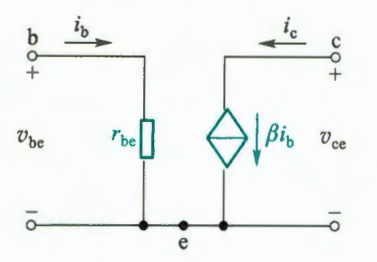
\includegraphics[width=0.3\linewidth]{pic/BJT的简化小信号模型.png}
    \caption{BJT的简化小信号模型\cite{康华光}\label{BJT的简化小信号模型}}
\end{figure}

\subsubsection{二、N型MOSFET的H参数小信号模型}
\textit{(本小节的内容仅做了解)}

NMOS的H参数小信号模型如图\ref{NMOS的简化小信号模型}所示,其中
\begin{equation}
    r_{\mathrm{ds}}\approx\frac{1}{\lambda i_{\mathrm{DQ}}}, g_\mathrm{m}=2\sqrt{K_{\mathrm{n}}i_{\mathrm{DQ}}},
\end{equation}
其中的参数$\lambda$来自沟道长度调制效应,实际中往往取$\lambda=0$。

\begin{figure}[htb]
    \centering
    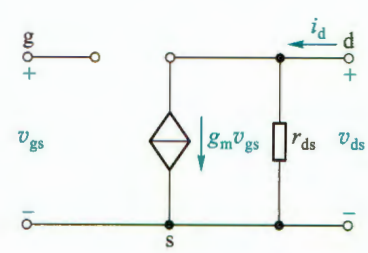
\includegraphics[width=0.3\linewidth]{pic/NMOS的简化小信号模型.png}
    \caption{NMOS的简化小信号模型\cite{康华光}\label{NMOS的简化小信号模型}}
\end{figure}

\subsubsection{三、利用小信号模型对放大电路的分析}
利用小信号模型分析放大电路的方法往往比较固定,一般情况下,按照固定的套路都能够解决问题。本节以BJT管为例,介绍如何利用小信号模型分析放大电路的基本套路。

\textbf{1.静态分析:}

\begin{itemize}
    \item 将电路中电容视为断路;
    \item 将BJT的发射结按照恒压降模型计算(对于硅管$V_{\mathrm{B}}-V_{\mathrm{E}}=\qty{0.7}{V}$);
    \item 寻找电压路径,使得该路径两端电压确定,且其中仅存在电阻和三极管(基极到发射极),并计算$I_{\mathrm{BQ}}$或者$I_{\mathrm{CQ}}$;
    \item 寻找电流路径,使得该路径两端电压确定,且其中仅存在电阻和三极管(集电极到发射极),并计算$V_{\mathrm{CEQ}}$。
\end{itemize}

\textbf{2.动态分析:}

\begin{itemize}
    \item 判断元件工作状态是否进入放大区;
    \item 利用三级管的$I_{\mathrm{EQ}}$计算动态参数$r_{\mathrm{be}}$;
    \item 将大电容(耦合电容和旁路电容)视为短路,直流信号源置零,并将三极管替换为小信号模型,计算所需要的结果。
\end{itemize}

\subsection{共射放大电路的分析}
本节通过两种不同的共射放大电路作为例题来介绍如何使用图解法和小信号模型法。

\subsubsection{一、图解法求解基本共射放大电路}

基本共射放大电路如图\ref{基本共射放大电路}所示,其中$v_{\mathrm{s}}$为待放大的时变输入信号。假设参数使BJT工作在放大区。

\begin{figure}[htb]
    \centering
    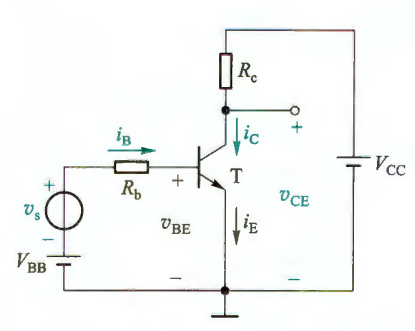
\includegraphics[width=0.55\linewidth]{pic/基本共射放大电路.png}
    \caption{基本共射放大电路\cite{康华光}\label{基本共射放大电路}}
\end{figure}

\textbf{1.静态工作点的分析}

由于电路中交流量叠加在直流量上,因此先考虑直流通路。令$v_{\mathrm{s}}=0$,则输入端的外电路特性曲线为$v_{\mathrm{BE}}=V_{\mathrm{BB}}-i_{\mathrm{B}}R_{\mathrm{b}}$。与输入特性曲线联立就能得到静态工作点Q以及电流$I_{\mathrm{BQ}}$。

类似地,在输出特性曲线上,画出$v_{\mathrm{CE}}=V_{\mathrm{CC}}-i_{\mathrm{C}}R_{\mathrm{c}}$,与$i_{\mathrm{B}}=I_{\mathrm{BQ}}$对应的特性曲线的交点就是静态工作点Q。

\begin{figure}[htb]
    \centering
    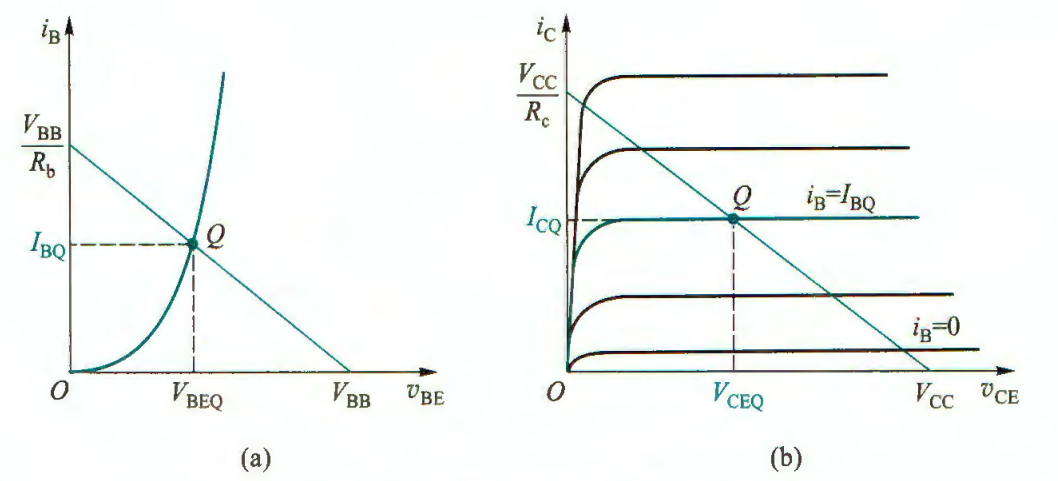
\includegraphics[width=0.8\linewidth]{pic/静态工作点的图解分析.png}
    \caption{静态工作点的图解分析\cite{康华光}\label{静态工作点的图解分析}}
\end{figure}

\textbf{2.动态参数的分析}

当$v_{\mathrm{s}}=V_{\mathrm{sm}}\sin \omega t$时,输入负载曲线为$v_{\mathrm{BE}}=V_{\mathrm{BB}}+v_{\mathrm{s}}-i_{\mathrm{B}}R_{\mathrm{b}}$,画出图像如图\ref{动态工作情况的图解分析1}所示,可以读出$i_{\mathrm{B}}$的波形。

类似地,可以在输出特性曲线上求出其他参数,如图\ref{动态工作情况的图解分析2}所示。

\begin{figure}[htb]
    \centering
        \subcaptionbox{输入回路\cite{康华光}\label{动态工作情况的图解分析1}}
        {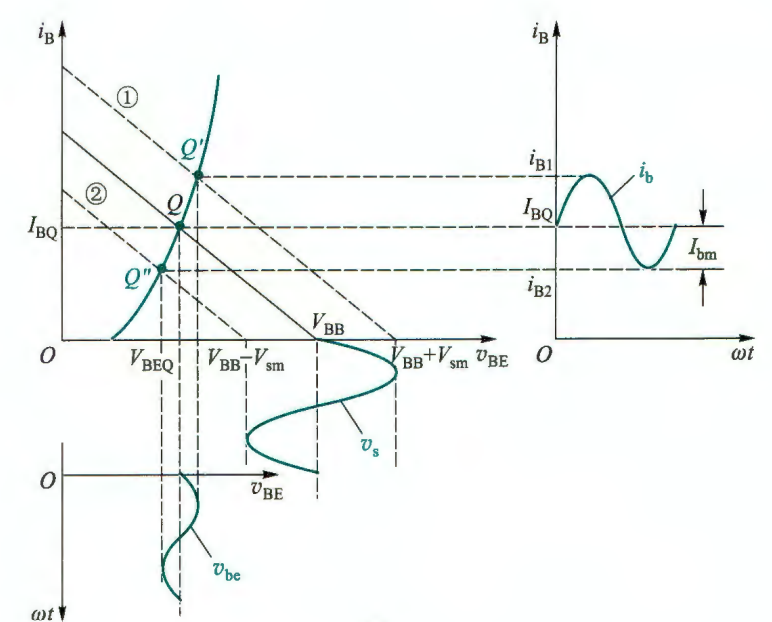
\includegraphics[width=0.45\textwidth]{pic/动态工作情况的图解分析1.png}}\qquad
        \subcaptionbox{输出回路\cite{康华光}\label{动态工作情况的图解分析2}}
        {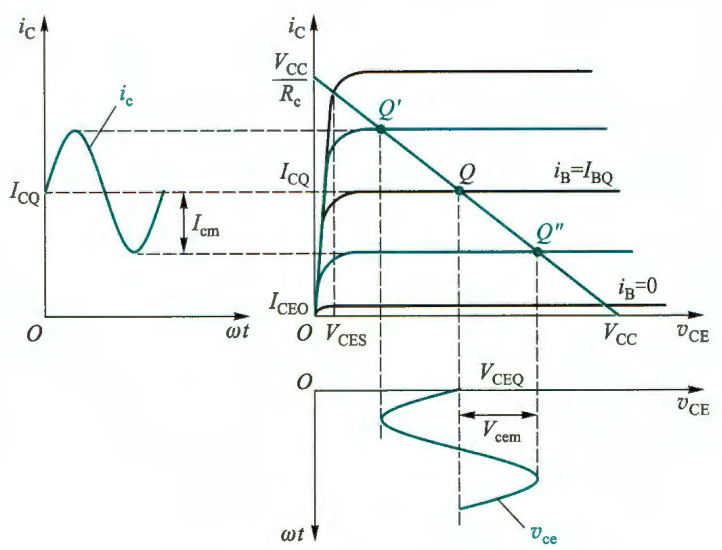
\includegraphics[width=0.45\textwidth]{pic/动态工作情况的图解分析2.png}}
        \caption{动态工作情况的图解分析\label{动态工作情况的图解分析}}
\end{figure}

\subsubsection{二、小信号模型法求解基极分压式射极偏置共射放大电路}

基极分压式射极偏置共射放大电路如图\ref{基极分压式射极偏置共射放大电路-电路图}所示。其中参数的选取需要使得电路满足$i_2\gg i_{\mathrm{B}}$,因此$i_1\approx i_{\mathrm{2}}$。

同时,选取合适的$R_{\mathrm{b1}}$、$R_{\mathrm{b2}}$和$R_{\mathrm{c}}$使得BJT工作在放大区。

\begin{figure}[htb]
    \centering
        \subcaptionbox{电路图\cite{康华光}\label{基极分压式射极偏置共射放大电路-电路图}}
        {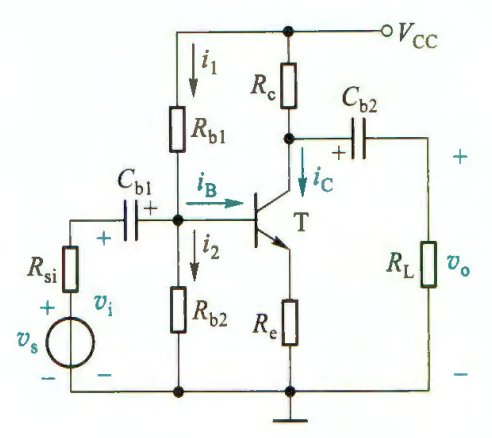
\includegraphics[width=0.4\textwidth]{pic/基极分压式射极偏置共射放大电路-无射极旁路电容.png}}\qquad
        \subcaptionbox{直流通路\cite{康华光}\label{基极分压射极偏置电路-直流通路}}
        {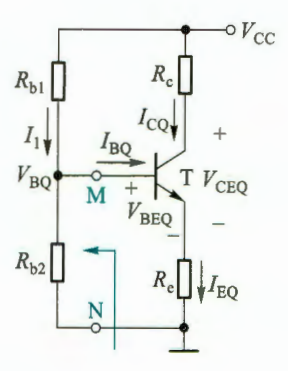
\includegraphics[width=0.28\textwidth]{pic/基极分压射极偏置电路-直流通路.png}}
        \caption{基极分压式射极偏置共射放大电路\label{基极分压式射极偏置共射放大电路}}
\end{figure}

\textbf{1.静态分析:}

断开$C_{\mathrm{b1}}$、$C_{\mathrm{b2}}$支路,得到图\ref{基极分压射极偏置电路-直流通路}。由于$i_1\approx i_{\mathrm{2}}$,因此
\begin{equation}
    V_{\mathrm{BQ}}=\frac{R_{\mathrm{b2}}}{R_{\mathrm{b1}}+R_{\mathrm{b2}}}V_{\mathrm{CC}}
\end{equation}

由此在经过基极b、发射极e和电阻$R_\mathrm{e}$的支路上,可以计算出
\begin{equation}
    I_{\mathrm{BQ}}=\frac{V_{\mathrm{BQ}}-V_{\mathrm{BEQ}}}{(1+\beta)R_{\mathrm{e}}}
\end{equation}

再代入\ref{公式-BJT的小信号模型}式,就能计算出小信号模型中的$r_\mathrm{be}$。

\textbf{2.动态分析:}

将所有电容短路,直流信号源置零,并将三极管替换为小信号模型,就能得到图\ref{基极分压射极偏置电路-交流通路}。

\begin{figure}[htb]
    \centering
    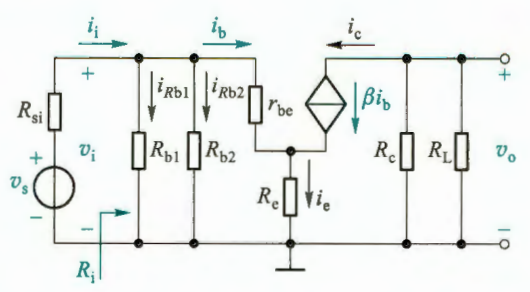
\includegraphics[width=0.5\linewidth]{pic/基极分压射极偏置电路-交流通路.png}
    \caption{基极分压式射极偏置共射放大电路的交流通路\cite{康华光}\label{基极分压射极偏置电路-交流通路}}
\end{figure}

因为有
\begin{align}
    v_\mathrm{o}=-\beta i_\mathrm{b} (R_\mathrm{c}\parallel R_\mathrm{L}) \\
    v_\mathrm{i}=(r_\mathrm{be}+(1+\beta)R_\mathrm{e})i_\mathrm{b}
\end{align}
所以电压增益为
\begin{equation}\label{公式-共射放大电路增益}
    A_v=\frac{v_\mathrm{o}}{v_\mathrm{i}}=-\frac{\beta (R_\mathrm{c}\parallel R_\mathrm{L})}{r_\mathrm{be}+(1+\beta)R_\mathrm{e}}
\end{equation}

对于输入电阻
\begin{equation}
    R_\mathrm{i}=R_\mathrm{b1} \parallel R_\mathrm{b2} \parallel (r_\mathrm{be}+(1+\beta)R_\mathrm{e})
\end{equation}

在计算输出电阻时,本身并没有电源在起作用。此时应该把将原来的独立源直接置零,并把输出网络的负载换成一个电源。在BJT电路中,$r_\mathrm{ce}$往往很大,因此上述电路的输出电阻
\begin{equation}
    R_\mathrm{o}=R_\mathrm{c}
\end{equation}

\section{BJT的三种基本放大电路}
晶体管组成的基本放大电路是由共射、共基、共集三种接法。要判断某个放大电路属于哪种类型,先判断输⼊和输出分别是哪⼀极,然后剩下那一极就是共什么极,如图\ref{BJT放大电路三种组态的性能}所示。

\begin{figure}[htb]
    \centering
    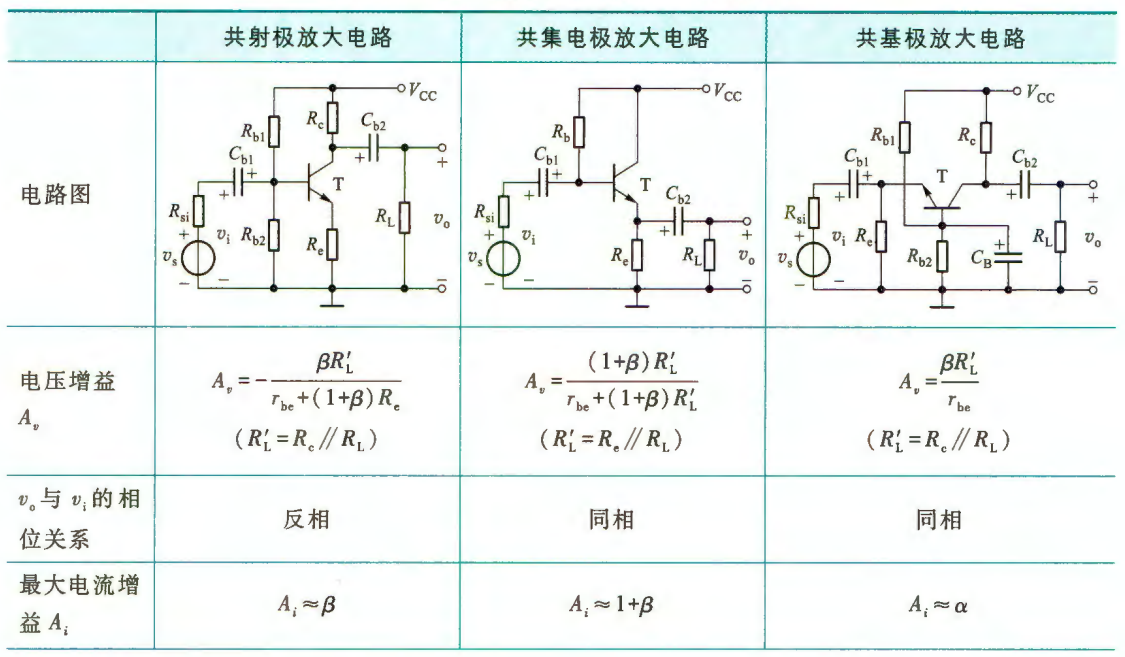
\includegraphics[width=0.9\linewidth]{pic/BJT三种类型的放大电路-1.png}
    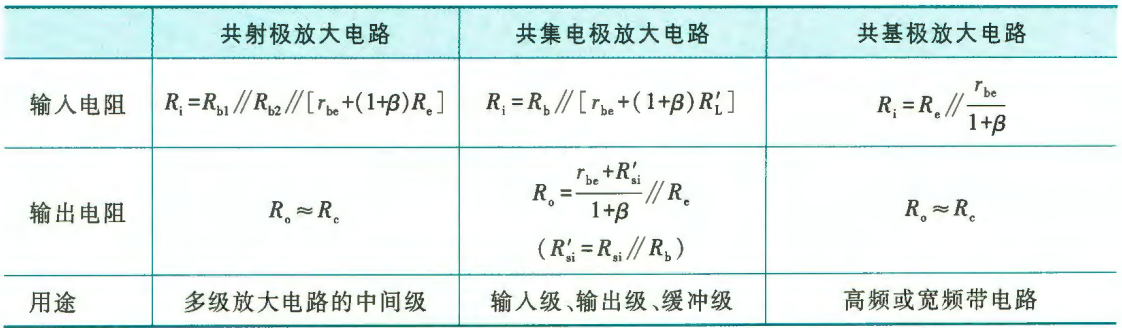
\includegraphics[width=0.9\linewidth]{pic/BJT三种类型的放大电路-2.png}
    \caption{BJT放大电路三种组态的性能\cite{康华光}\label{BJT放大电路三种组态的性能}}
\end{figure}

当掌握基本分析方法后,可以通过对这三种电路的分析加深印象。由于教材5.2.4节和5.2.5节有详细的推导,此处从略,仅提供基本结论。

1.基本共射放大电路既能放大电流又能放大电压,常作为低频放大电路的单元电路。

2.基本共集放大电路只能放大电流不能放大电压,输入电阻大,输出电阻小,有电压跟随的特点。

3.基本共基放大电路只能放大电压不能放大电流,有电压跟随的特点。
    \chapter{集成运算放大电路}
除了放大模拟信号,也需要对信号进行各种运算。而基本放大电路难以实现这些运算,因此引入多级放大电路,并制成了集成运算放大器。本章将会先简单介绍多级放大电路,然后介绍集成运放对每一级相应的电路,最后讲解对集成运放的特性及运算电路。

\section{多级放大电路}
放大电路中每一个基本放大电路称为一级,而将它们连接起来就称为\textbf{级间耦合}\index{J!级间耦合}。

\subsection{耦合方式}

\subsubsection{一、直接耦合}
最简单的连接方式就是将前一级的输出端直接连接到后一级的输入端,这种称为\textbf{直接耦合}\index{Z!直接耦合}。由于各级之间是直接连接起来的,静态工作点会相互影响,且存在零漂现象。

\subsubsection{二、阻容耦合}
为了避免静态工作点相互影响,会使用电容连接电路的两级,称为\textbf{阻容耦合}\index{Z!阻容耦合}。由于存在电容,会导致低频信号难以通过,且难以集成到一片硅片上。

\subsection{多级放大电路的动态分析}
多级放大电路的电压放大倍数就是各级电压放大倍数的乘积,其中值得注意的是,每一级的放大倍数应当是以后级的输入电阻作为负载时的放大倍数。多级放大电路的输入电阻就是第一级的输入电阻,而输出电阻就是最后一级的输出电阻。

在计算的过程中,需要注意必须将第二级的输入电阻作为第一级的负载,计算在第一级的增益之内。

\section{电流源电路}
在集成电路中,制作一个三极管比制作一个电阻所占用的面积更小,因此往往会选择三极管构成直流电流源,常用于在电路中提供静态偏置,或者充当大电阻。

\subsection{镜像电流源}\index{J!镜像电流源}
图\ref{BJT镜像电流源电路}为BJT镜像电流源电路。对静态工作点进行分析,可以得到\textbf{基准电流}\index{J!基准电流}
\begin{equation}
    I_{\mathrm{REF}}=\frac{V_{\mathrm{CC}}-V_{\mathrm{BE}}-(-V_{\mathrm{EE}})}{R}
\end{equation}

由对称性和节点电流法,可以得到
\begin{equation}
    I_\mathrm{O}=I_{\mathrm{C2}}=\frac{I_{\mathrm{REF}}}{1+2/\beta}
\end{equation}

可见,电流大小与负载无关。而其输出电阻为
\begin{equation}
    r_{\mathrm{o}}=r_{\mathrm{ce2}}=\frac{1}{\lambda I_{\mathrm{C2}}}
\end{equation}

因此其输出电阻很大,可以在电路中取代大电阻。

实际上,在$V_{\mathrm{CC}}$一定的情况下,如果要求$I_{\mathrm{C2}}$很大,则需要$I_{\mathrm{REF}}$很大,导致电阻上的功耗增加,这应当避免。如果要求$I_{\mathrm{C2}}$很小,则需要$I_{\mathrm{REF}}$很小,此时需要电阻$R$很大,也应当避免。因此派生了其他类型的电流源。

\begin{figure}[htb]
    \centering
    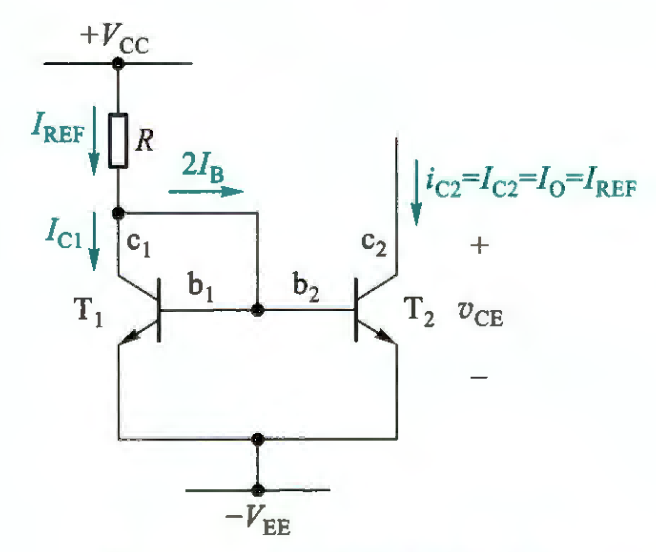
\includegraphics[width=0.5\linewidth]{pic/BJT镜像电流源电路.png}
    \caption{BJT镜像电流源电路\cite{康华光}\label{BJT镜像电流源电路}}
\end{figure}

\subsection{比例电流源}
\textit{(本节的内容仅做了解)}

比例电流源如图\ref{比例电流源}所示。由电路可知
\begin{equation}
    V_{\mathrm{BE0}}+I_{\mathrm{E0}}R_{\mathrm{e0}}=V_{\mathrm{BE1}}+I_{\mathrm{E1}}R_{\mathrm{e1}}
\end{equation}

而BJT管的发射结电压和发射结电流之间的关系近似为(这里不再使用恒压降模型)
\begin{equation}
    V_{\mathrm{BE}}=V_{\mathrm{T}}\ln \frac{I_{\mathrm{E}}}{I_{\mathrm{S}}}
\end{equation}

其中$V_{\mathrm{T}}$为电压当量,因此
\begin{equation}
    I_{\mathrm{E1}}R_{\mathrm{e1}}-I_{\mathrm{E0}}R_{\mathrm{e0}}\approx V_{\mathrm{T}}\ln \frac{I_{\mathrm{E0}}}{I_{\mathrm{E1}}}
\end{equation}

由于$I_{\mathrm{C0}}\approx I_{\mathrm{E0}}\approx I_{\mathrm{R}}$,$I_{\mathrm{C1}}\approx I_{\mathrm{E1}}$,则
\begin{equation}
    I_{\mathrm{C1}}\approx \frac{R_{\mathrm{e0}}}{R_{\mathrm{e1}}}I_\mathrm{R}+\frac{V_{\mathrm{T}}}{R_{\mathrm{e1}}}\ln \frac{I_{\mathrm{R}}}{I_{\mathrm{C1}}}
\end{equation}

在一定范围内,对数项可以忽略,因此$I_{\mathrm{C1}}$与$I_{\mathrm{R}}$成正比。只要改变$R_{\mathrm{e0}}$和$R_{\mathrm{e1}}$的关系,就可以改变$I_{\mathrm{C1}}$与$I_{\mathrm{R}}$的比例关系。

\begin{figure}[htb]
    \centering
    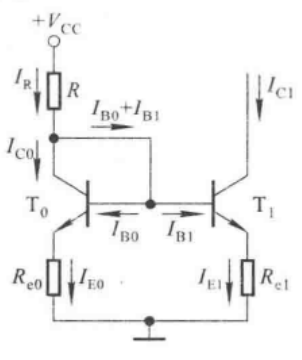
\includegraphics[width=0.3\linewidth]{pic/比例电流源.png}
    \caption{比例电流源\cite{华成英}\label{比例电流源}}
\end{figure}

\subsection{微电流源}
在比例电流源的基础上取$R_{\mathrm{e0}}=0$,就构成了微电流源。

\section{差分放大电路}
由于阻容耦合中会出现大量的电容,不便于集成,因此在集成电路中仍会采用直接耦合的方式,但直接耦合会产生零点漂移的现象。\textbf{零点漂移}\index{L!零点漂移},顾名思义,就是输入电压被置零但输出电压随时间变化的现象。

后来,人们想出了一个对称的构造——差分放大电路,并将其作为集成放大电路的输入级,有效地抑制了零点漂移的现象。本节仅讨论BJT构成的差分放大电路。

\subsection{差模信号与共模信号及相关参数}
差分放大电路的整体结构非常对称,这样就消除了各种各样的干扰和噪声。各种干扰的信号由于是对两边同步输入就变成了共模信号,在输出时一作差就被消除了,而需要的信号变成了差模信号。为了更好地讨论差分放大电路的性能,引入如下概念。

\subsubsection{一、信号}
在电路中,信号有两个输入端:同相输入端$v_{\mathrm{P}}$和反相输入端$v_{\mathrm{N}}$,其中下标字母P和N分别表示positive和negative。

另一种分类方式为差模信号和共模信号,其定义如下:

1.\textbf{差模信号}\index{X!信号!差模信号}:定义为两输入端信号的差值,即$v_{\mathrm{id}}=v_{\mathrm{P}}-v_{\mathrm{N}}$,其中下标字母d的含义为differential。

2.\textbf{共模信号}\index{X!信号!共模信号}:定义为两输入端信号的算数平均值,即$v_{\mathrm{ic}}=(v_{\mathrm{P}}+v_{\mathrm{N}})/2$,其中下标字母c的含义为common。

\subsubsection{二、增益}
1.\textbf{差模电压增益}\index{F!放大倍数!差模电压增益}:即仅考虑差模信号输入时的电压增益$A_{\mathrm{vd}}=v_{\mathrm{od}}/v_{\mathrm{id}}$。

2.\textbf{共模电压增益}\index{F!放大倍数!共模电压增益}:即仅考虑共模信号输入时的电压增益$A_{\mathrm{vc}}=v_{\mathrm{oc}}/v_{\mathrm{ic}}$。

则总输出为
\begin{equation*}
    v_\mathrm{o}=v_\mathrm{od}+v_\mathrm{oc}=A_\mathrm{vd}v_\mathrm{id}+A_\mathrm{vc}v_\mathrm{ic}
\end{equation*}

\subsubsection{三、共模抑制比}
为了反映电路放大差模信号和抑制共模信号的综合能力,引入\textbf{共模抑制比}\index{G!共模抑制比}$K_{\mathrm{CMR}}=|A_{\mathrm{vd}}/A_{\mathrm{vc}}|$,下标CMR表示common mode rejection。

另外需要注意的是,\textbf{这里讨论的输入信号都是交流小信号},而非直流信号。

\subsection{差分放大电路的分析}
差分放大电路特殊的地方在于它的两个输入端都是有效输入端,而非一个输入端接地,这也导致其分为双端输入和单端输入。实际上,差分放大电路的输入和输出都可以有单端和双端两种,因此一共有四种组合。

通常,两个BJT的射极会接在同一个恒流源(如镜像电流源),导致电路中看起来有很多管子。但其实只要按照功能将一个个模块分解开就知道并不复杂。

\subsubsection{一、静态分析}
在静态分析的时候直接将两个基极接地即可。由于发射极接了恒流源,静态分析并不困难,此处从略。

\subsubsection{二、动态分析}
在动态分析的时候,通常需要将共模信号和差模信号分开讨论。

\begin{figure}[htb]
    \centering
        \subcaptionbox{输入差模信号时\cite{康华光}\label{输入差模信号时的交流通路}}
        {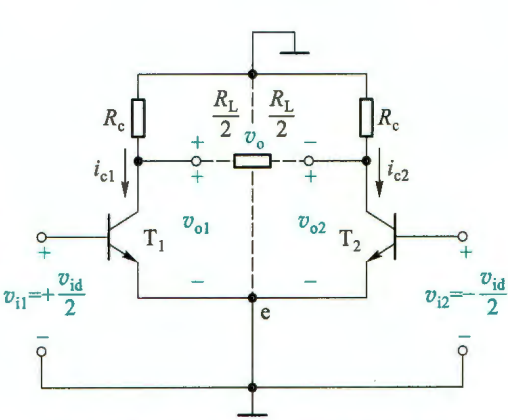
\includegraphics[width=0.45\textwidth]{pic/输入差模信号时的交流通路.png}}\qquad
        \subcaptionbox{输入共模信号时\cite{康华光}\label{输入共模信号时的交流通路}}
        {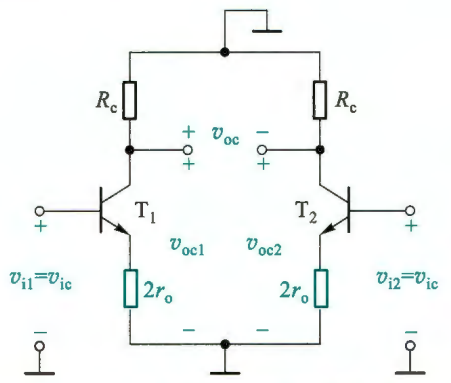
\includegraphics[width=0.45\textwidth]{pic/输入共模信号时的交流通路.png}}
        \caption{输入不同信号时的交流通路\label{输入不同信号时的交流通路}}
\end{figure}

\textbf{1.差模信号的增益}

输入差模信号时的交流通路如图\ref{输入差模信号时的交流通路}所示。在分析差模信号时,考虑到电路理想对称,对称轴上电压为0,相当于全部接地。

a.双端输入、单端输出时

不接负载时,在$v_{\mathrm{o1}}$端输出的电压增益为
\begin{equation}
    A_{v\mathrm{d1}}=-\frac{\beta R_\mathrm{c}}{2r_\mathrm{be}}
\end{equation}

接上负载后$R_\mathrm{L}$,在$R_\mathrm{c}$上并上负载电阻$R_\mathrm{L}$即可。

对于差模电压增益,从两个口输出的区别在于其相位不同,相差一个负号。

b.双端输入、双端输出时

在不接负载的情况下,双端输出的差模电压增益是单端输出的2倍,与单管的电路增益相同,相当于用双倍的元件换取了抑制零漂的能力。虽然它的差模增益更高,但是没有对地输出使得它不如单端输出稳定。

如果接上负载,利用对称性,等效于单边并上了一个$R_\mathrm{L}/2$的电阻,电压增益为
\begin{equation}
    A_{v\mathrm{d}}=-\frac{\beta R_\mathrm{c} \parallel (R_\mathrm{L}/2)}{r_\mathrm{be}}
\end{equation}

c.单端输入时

差模信号的单端输入必然伴随着共模信号的输入。单端输入可以等效为双端输入,因此单端输入和双端输入的差模增益指标相同。

\textbf{2.共模信号的增益}

输入共模信号时,由于此时射极电压不再为0,电流源的内阻不可忽略。如果保持射极电压不变,可以将$r_\mathrm{o}$分别等效到两端支路上,如图\ref{输入共模信号时的交流通路}所示。

由于共模输入两端信号完全相同,输入时没有单端输入和双端输入之分。

a.双端输出时

由于两边完全对称,共模电压增益为0,共模抑制比$K_{\mathrm{CMR}}=\infty$。

b.单端输出时

共模电压增益类似基本共射放大电路的电压增益,只是将$R_\mathrm{e}$替换为了$2r_\mathrm{o}$:
\begin{equation}
    A_{v\mathrm{c}}=-\frac{\beta R_\mathrm{c}}{r_\mathrm{be}+(1+\beta)2r_\mathrm{o}}\approx -\frac{R_\mathrm{c}}{2r_\mathrm{o}}
\end{equation}
此时共模抑制比$K_{\mathrm{CMR}}$有限。

\textbf{3.输入电阻和输出电阻}

差模输入电阻
\begin{equation}
    R_\mathrm{id}=2r_\mathrm{be}
\end{equation}

共模输入电阻
\begin{equation}
    R_\mathrm{ic}=\frac{1}{2}[r_\mathrm{be}+(1+\beta)(2r_\mathrm{o})]
\end{equation}

单端输出时的输出电阻
\begin{equation}
    R_\mathrm{o}=R_\mathrm{c}
\end{equation}

双端输出时的输出电阻是单端输出的两倍
\begin{equation}
    R_\mathrm{o}=2R_\mathrm{c}
\end{equation}

\textbf{实际上,对于这些结论,只要按照之前的动态分析方法,将BJT替换为相应的小信号模型就能直接算出来。}图\ref{差分放大电路四种接法的比较}中汇总了几种电路相关结论,注意原来的直流源被替换成了射极电阻$R_\mathrm{e}$。

\begin{figure}[htb]
    \centering
    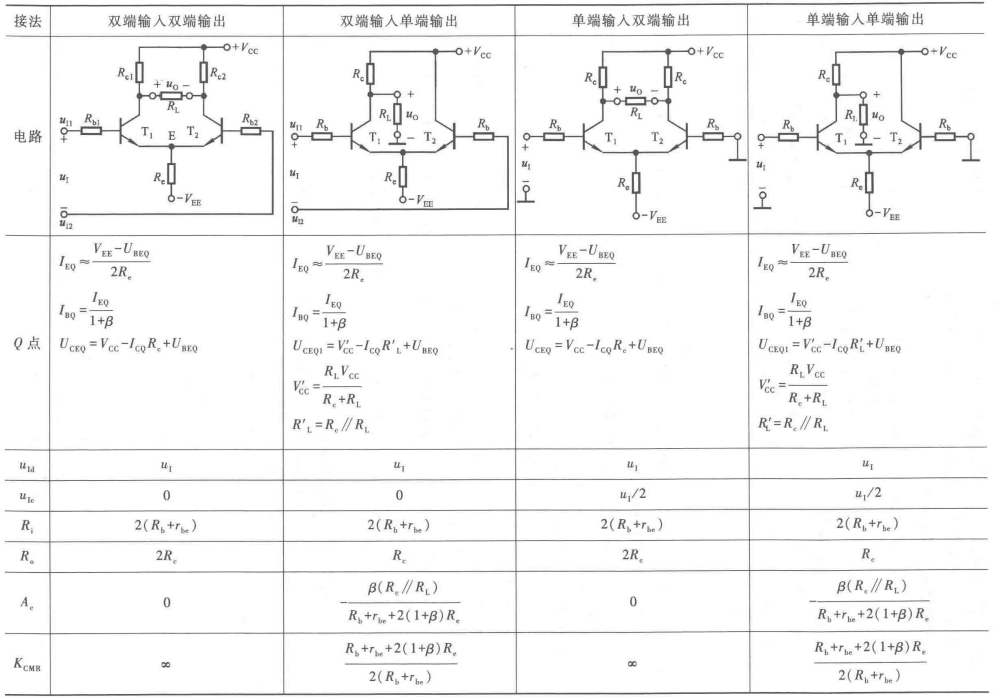
\includegraphics[width=0.95\linewidth]{pic/差分放大电路四种接法的比较.png}
    \caption{差分放大电路四种接法的比较(图片来源:康华光指导92页)\label{差分放大电路四种接法的比较}}
\end{figure}

\section{直接耦合互补输出级}
\textit{(本节的内容仅做了解)}
上一节讲解的差分放大器,往往用于多级放大电路的输入级,将零漂扼杀于摇篮之中。而在输出级,一般要求输出电阻低,且最大不失真输出电压尽可能大,因此产生了直接耦合互补输出级。如图\ref{互补射极输出电路}所示。互补输出级也常作为功率放大电路。

\begin{figure}[htb]
    \centering
    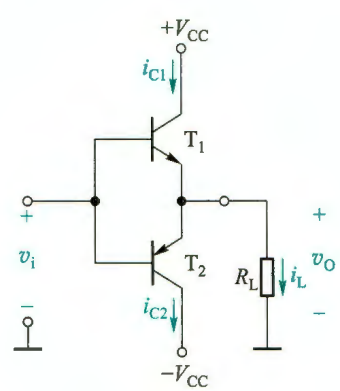
\includegraphics[width=0.25\linewidth]{pic/互补射极输出电路.png}
    \caption{互补射极输出电路\cite{康华光}\label{互补射极输出电路}}
\end{figure}

\section{集成运算放大器}
将上述各单元电路组合起来,就可以构成一个\textbf{集成电路运算放大器},简称为\textbf{集成运放}。

集成运放通常由至少三级放大电路构成。比较常见的构成是,输入级为CMOS差分放大电路作为输入,中间级为共射放大电路,输出为功率放大电路作为输出。其中,第一级将电路的两个输入端口作差抑制共模信号,第二级让信号放大,第三级再次放大并且提供比较好的输出匹配。这样就得到了一个输入电阻高、输出电阻低、增益系数大的放大电路模块。

集成运放由于其近似理想的特性备受关注,并且多用于各种模拟信号的运算。由于其内部结构复杂,本节将集成运放作为一个黑匣子,讨论集成运放的外部特性,并简单介绍集成运放的应用电路。

\subsection{运算放大器的特性}
运算放大电路的简化模型如图\ref{运算放大器的电路简化模型}所示,其中供电电源通常会被省略,只会在必要时画出。

\begin{figure}[htb]
    \centering
    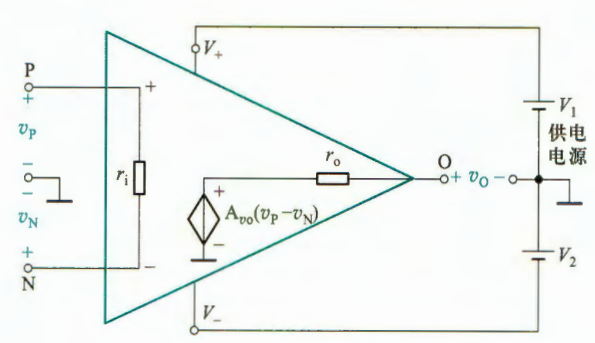
\includegraphics[width=0.55\linewidth]{pic/运算放大器的电路简化模型.png}
    \caption{运算放大器的电路简化模型\cite{康华光}\label{运算放大器的电路简化模型}}
\end{figure}

由于输入级为差分放大电路,输出电压与输入级电压之差成正比,即$v_{\mathrm{O}}=A_{v\mathrm{o}}(v_{\mathrm{P}}-v_{\mathrm{N}})$。其中$A_{v\mathrm{o}}$为\textbf{开环电压增益}\index{K!开环电压增益},而P表示\textbf{同相输入端}\index{S!输入端!同相输入端},N表示\textbf{反相输入端}\index{S!输入端!反相输入端}。此外,在图\ref{运算放大器的电路简化模型}中还可以看到输入电阻$r_\mathrm{i}$和输出电阻$r_\mathrm{o}$。

但实际上,由于工作电源的限制,\textbf{线性工作区}\index{X!线性工作区}很小。当$A_{v\mathrm{o}}(v_{\mathrm{P}}-v_{\mathrm{N}})$过大时,会进入\textbf{饱和区}\index{B!(集成运放)饱和区}。

对于集成运放,同样有差模信号、共模信号、共模抑制比等等定义,可以直接类比差分放大电路对应的概念。由于输出电压只与差模信号有关,因此共模电压增益为0,共模抑制比为无穷。

\subsection{理想运算放大器}
为了简化电路分析,人们将集成运放的各项指标理想化,就能得到理想的运放模型。

对于理想的运算放大器,最重要的两个性质为:

1.开环电压增益$A_{v\mathrm{o}}=\infty$,但输出电压为有限值,因此$v_{\mathrm{P}}=v_{\mathrm{N}}$,称为“\textbf{虚短}”。

2.输入电阻$r_{\mathrm{i}}=\infty$,此时$i_{\mathrm{P}}=i_{\mathrm{N}}=0$,称为“\textbf{虚断}”。

此外,还会认为其输出电阻$r_{\mathrm{o}}=0$。

\subsection{运算放大器的应用电路}
由于集成运放的开环增益极高,线性区$(v_{\mathrm{P}}-v_{\mathrm{N}})$非常小,难以保证其工作在线性区,因此需要引入负反馈来减小$(v_{\mathrm{P}}-v_{\mathrm{N}})$的值,也就是让其工作在闭环状态。

本节仅简单讨论最基本的运放应用电路之一——同相放大电路,如图\ref{同相放大电路}所示。

\begin{figure}[htb]
    \centering
    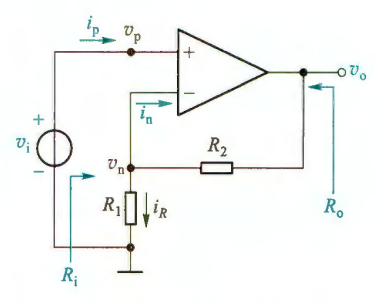
\includegraphics[width=0.45\linewidth]{pic/同相放大电路.png}
    \caption{同相放大电路\cite{康华光}\label{同相放大电路}}
\end{figure}

在运放的反相端运用KCL,得到
\begin{equation}
    \frac{v_\mathrm{o}-v_\mathrm{n}}{R_2}=\frac{v_\mathrm{n}}{R_1}+i_\mathrm{n}
\end{equation}

再利用$v_{\mathrm{p}}=v_{\mathrm{n}}=v_{\mathrm{i}}$和$i_{\mathrm{p}}=i_{\mathrm{n}}=0$,就得到
\begin{equation}
    A_v=1+\frac{R_2}{R_1}
\end{equation}

除了同相放大电路外,还有以下基本应用:
\begin{itemize}
    \item 反相放大电路;
    \item 电压跟随器(缓冲器、隔离器);
    \item 求和电路、求差电路;
    \item 积分电路、微分电路;
\end{itemize}

此外,还有更复杂的对数电路、指数电路、乘法电路、除法电路……
    \chapter{放大电路中的反馈}
在电路中引入负反馈后,也可以使得电路保持稳定,并取得一些其他意想不到的效果。
\section{反馈的基本概念与分类}
\subsection{反馈的基本概念}
\textbf{反馈}是指电路的输出量的一部分或者全部通过一定的电路形式作用到输入回路,以影响输入量。
\begin{figure}[htb]
    \centering
    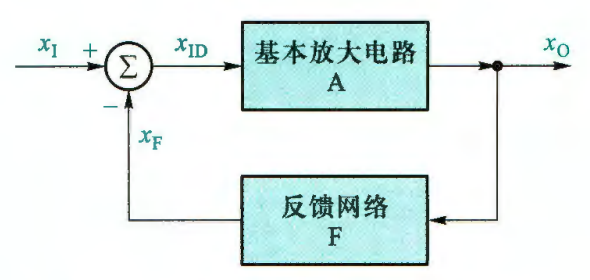
\includegraphics[width=0.5\linewidth]{pic/反馈.png}
    \caption{反馈放大电路的方框图\cite{康华光}\label{反馈}}
\end{figure}

其中$x_{\mathrm{I}}$表示输入信号,$x_{\mathrm{O}}$表示输出信号,$x_{\mathrm{ID}}$表示净输入信号,$x_{\mathrm{F}}$表示反馈信号。而\textbf{基本放大电路增益}为$A=x_{\mathrm{O}}/x_{\mathrm{ID}}$,\textbf{反馈系数}$F=x_{\mathrm{F}}/x_{\mathrm{O}}$。

\subsection{基本反馈的分类与判断}\label{基本反馈的分类与判断}
\subsubsection{一、开环与闭环}
若没有反馈网络,称为\textbf{开环}\index{K!开环},而如果存在反馈网络,则称为\textbf{闭环}\index{B!闭环}。

判断电路中有无反馈只需要看有无将输出回路和输入回路相连接的通路即可。

\subsubsection{二、级内反馈和级间反馈}
每级各自存在的反馈就是\textbf{级内反馈}\index{F!反馈!级内反馈},跨级的反馈就是\textbf{级间反馈}\index{F!反馈!级间反馈}。

\subsubsection{三、直流反馈和交流反馈}
存在于直流通路中的反馈称为\textbf{直流反馈}\index{F!反馈!直流反馈},而存在于交流通路中的反馈称为\textbf{交流反馈}\index{F!反馈!交流反馈}。

\subsubsection{四、正反馈和负反馈}
使净输入量变大的反馈称为\textbf{正反馈}\index{F!反馈!正反馈},使净输入量变小的反馈称为\textbf{负反馈}\index{F!反馈!负反馈}。

常用方法为“瞬时极性法”:首先假设瞬时极性增加,用(+)标出,然后沿着信号传输的路径判断有关节点电压的瞬时值。若增强输入信号就为正反馈,否则为负反馈。

\begin{figure}[htb]
    \centering
    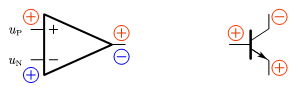
\includegraphics[width=0.5\linewidth]{pic/反馈极性的判断.png}
    \caption{常用元件反馈极性的判断\label{反馈极性的判断}}
\end{figure}

\section{负反馈放大电路的四种组态及判断}
除了\ref{基本反馈的分类与判断}小节中提到的四种分类方法,反馈电路还可以分为串联/并联反馈和电压/电流反馈,而这两种分类通常是对\textbf{交流负反馈}放大电路而言的,非常重要,因此独成一节。

\subsection{串联反馈和并联反馈}
根据在反馈网络的输出端口和基本放大电路的输入端口的连接方式来判定。凡是反馈网络的输出端口与基本放大电路的输入端口串联连接的,为\textbf{串联反馈}\index{F!反馈!串联反馈};凡是反馈网络的输出端口与基本放大电路的输入端口并联连接的,为\textbf{并联反馈}\index{F!反馈!并联反馈}。

由定义可以知道,串联/并联反馈反映的是输入信号和反馈信号的叠加方式,而两个可以叠加的信号一定具有相同的量纲。因此,如果两个信号都是电压信号,则只能进行“串联”;如果两个信号都是电流信号,则只能进行“并联”(类比串联分压,并联分流)。

由上面的讨论可以得到一个快捷的判断方式:当反馈信号与输入信号接入不同端时,二者无法进行电流的叠加,叠加的是电压信号,是串联反馈;而当反馈信号与输入信号接入相同端时,可以进行电流的叠加,是并联反馈。

\begin{figure}[htb]
    \centering
    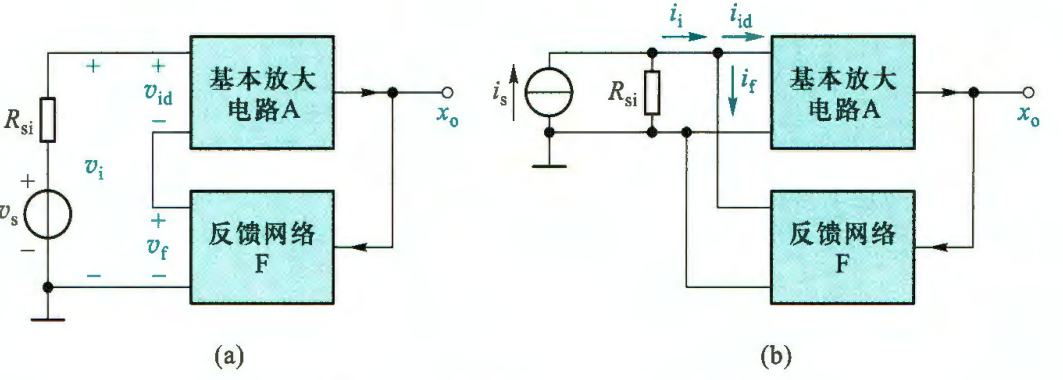
\includegraphics[width=0.75\linewidth]{pic/串联反馈和并联反馈.png}
    \caption{串联反馈和并联反馈(a)串联反馈(b)并联反馈\cite{康华光}\label{串联反馈和并联反馈}}
\end{figure}

\subsection{电压反馈和电流反馈}
根据在反馈网络的输入端口和基本放大电路的输出端口的取样对象来判定。

当反馈信号和输出电压成比例,为\textbf{电压反馈}\index{F!反馈!电压反馈};若与电流成比例,为\textbf{电流反馈}\index{F!反馈!电流反馈}。

当网络存在负反馈时,必定是电压反馈和电流反馈其中的一种。因此有一种特殊的判定方法——“输出短路法”。当输出电压$v_\mathrm{o}=0$时,反馈信号也不存在了,则反馈信号与输出电压成比例,为电压反馈,否则为电流反馈。

\begin{figure}[htb]
    \centering
    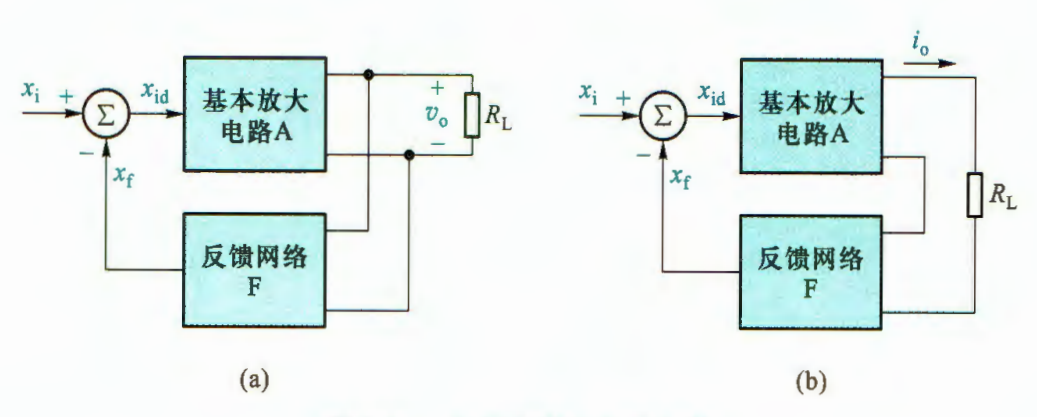
\includegraphics[width=0.75\linewidth]{pic/电压反馈和电流反馈.png}
    \caption{电压反馈和电流反馈(a)电压反馈(b)电流反馈\cite{康华光}\label{电压反馈和电流反馈}}
\end{figure}

此外,反馈信号取自于谁,就可以稳定谁。电压负反馈可以稳定输出电压,电流负反馈可以稳定输出电流。

\subsection{四种组态的负反馈放大电路}
由上述两种分类进行两两组合,就可以得到四种组态的放大电路,即电压串联、电流串联、电压并联、电流并联。

在实际中,往往会根据不同的需求来决定采用哪种放大电路。电路中究竟应该引入串联反馈还是并联反馈,取决于输入信号是恒压源还是恒流源;而应该引入电压反馈还是电流反馈,取决于负载需要的是稳定的电压信号还是电流信号。

\subsection{负反馈放大电路增益的一般表达式}
负反馈放大电路组成的框图如图\ref{负反馈放大电路的组成框图}所示。

\begin{figure}[htb]
    \centering
    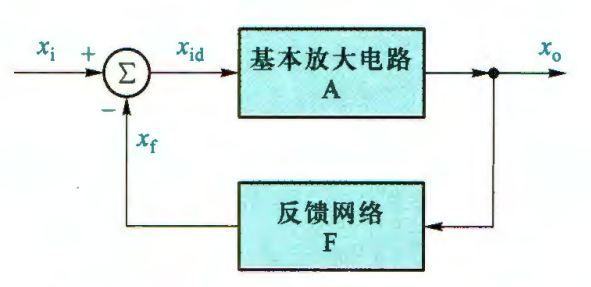
\includegraphics[width=0.5\linewidth]{pic/负反馈放大电路的组成框图.png}
    \caption{负反馈放大电路的组成框图\cite{康华光}\label{负反馈放大电路的组成框图}}
\end{figure}

其中$x_{\mathrm{i}}$表示输入信号,$x_{\mathrm{o}}$表示输出信号,$x_{\mathrm{id}}=x_{\mathrm{i}}-x_{\mathrm{f}}$表示净输入信号,$x_{\mathrm{f}}$表示反馈信号。

\textbf{基本放大电路增益(开环增益)}为$A=x_{\mathrm{o}}/x_{\mathrm{id}}$,\textbf{反馈系数}$F=x_{\mathrm{f}}/x_{\mathrm{o}}$,而\textbf{负反馈放大电路的增益(闭环增益)}为$A_{\mathrm{f}}=x_{\mathrm{o}}/x_{\mathrm{i}}$。

则可以得到闭环增益的一般表达式
\begin{equation}\label{闭环增益}
    A_{\mathrm{f}}=\frac{Ax_{\mathrm{id}}}{x_{\mathrm{id}}+AFx_{\mathrm{id}}}=\frac{A}{1+AF},
\end{equation}

其中,$AF$被称为\textbf{环路增益}\index{H!环路增益},$(1+AF)$被称为\textbf{反馈深度}\index{F!反馈!反馈深度}。可以看到,引⼊负反馈后电路增益降低,倍数与反馈深度有关。

\subsection{负反馈对放大电路性能的影响}

\subsubsection{一、提高增益的稳定性}
根据计算可以得到
\begin{equation}
    \frac{\mathrm{d}A_{\mathrm{f}}}{A_{\mathrm{f}}}=\frac{1}{1+AF}\frac{\mathrm{d}A}{A}
\end{equation}

可见,$A_{\mathrm{f}}$的稳定性是$A$的$(1+AF)$倍。

\subsubsection{二、对输入输出电阻的影响}
1.串联负反馈增大输入电阻:$R_\mathrm{if}=(1+AF)R_\mathrm{i}$。

2.并联负反馈减小输入电阻:$R_\mathrm{if}=R_\mathrm{i}/(1+AF)$。

3.电压负反馈减小输出电阻:$R_\mathrm{of}=R_\mathrm{o}/(1+AF)$。

4.电流负反馈增大输出电阻:$R_\mathrm{of}=(1+AF)R_\mathrm{o}$。

\subsubsection{三、减小非线性失真}

\subsubsection{四、抑制反馈环内噪声}

\subsubsection{五、扩展带宽}

虽然引入负反馈减小了增益,但整体来说,负反馈是利大于弊的。

\begin{figure}[htb]
    \centering
    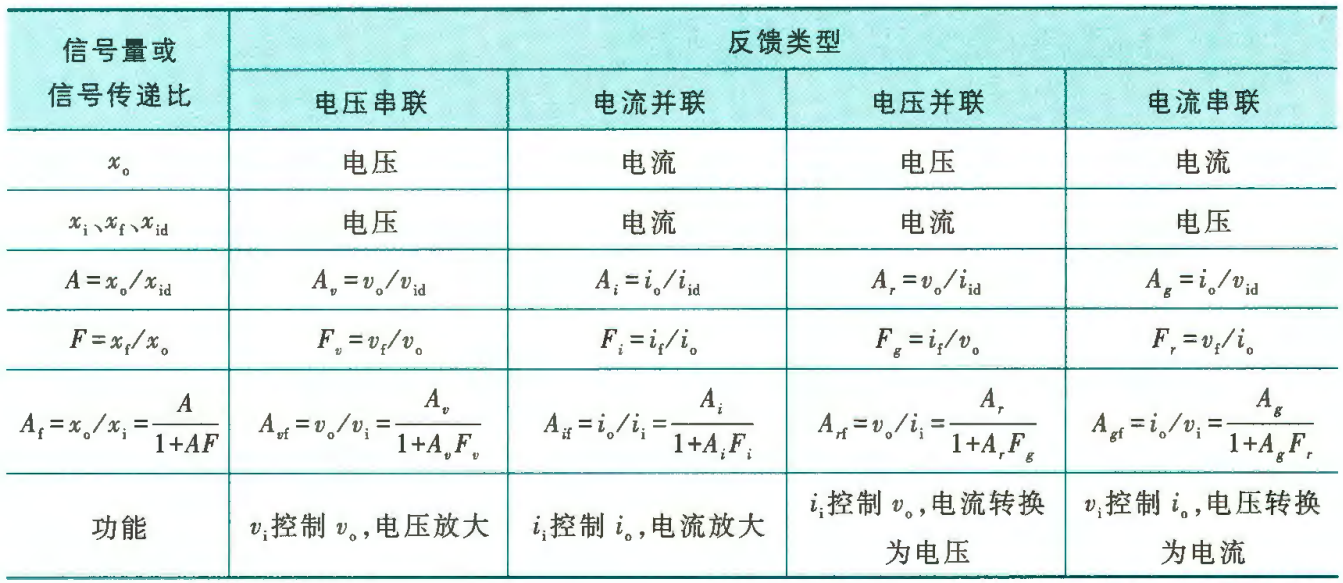
\includegraphics[width=0.99\linewidth]{pic/负反馈放大电路中各种信号量的含义.png}
    \caption{负反馈放大电路中各种信号量的含义\cite{康华光}\label{负反馈放大电路中各种信号量的含义}}
\end{figure}

\section{深度负反馈}
当$(1+AF)\gg 1$时,称为\textbf{深度负反馈}\index{F!反馈!深度负反馈},此时
\begin{equation}
    A_{\mathrm{f}}=\frac{1}{F},
\end{equation}

可以看到,闭环增益只取决于反馈系数,与开环增益无关。本质上,深度负反馈是将\ref{闭环增益}中分母上的净输入量$x_{\mathrm{id}}$忽略了。

无论是串联反馈还是并联反馈,只要在深度负反馈的条件下,均有$v_{\mathrm{id}}=0$(虚短)和$i_{\mathrm{id}}=0$(虚断)同时存在。利用这两个性质可以很方便地求出负反馈电路的闭环增益。

    \appendix
    \chapter{放大电路的构建}
\textit{(本章的内容仅做了解)}

通过对BJT原理的分析,可以知道当BJT工作在放大区时,基极上一个很小的电流就可以引起集电极上一个较大电流的变化。本章将通过一个例子来说明如何利用这个特性来构造一个合理的放大电路。

\section{基本共射放大电路的构成}
想要利用BJT的放大特性来放大一个小信号,最简单的想法就是直接在BJT将信号源直接接在射极的两端,如图\ref{1}所示。但是实际中,$v_\mathrm{i}$的量级一般都是毫伏甚至更小,这样直接加在两端会导致发射结无法正偏。此时BJT没有工作在放大区,无法放大。

\begin{figure}[htb]
    \centering
    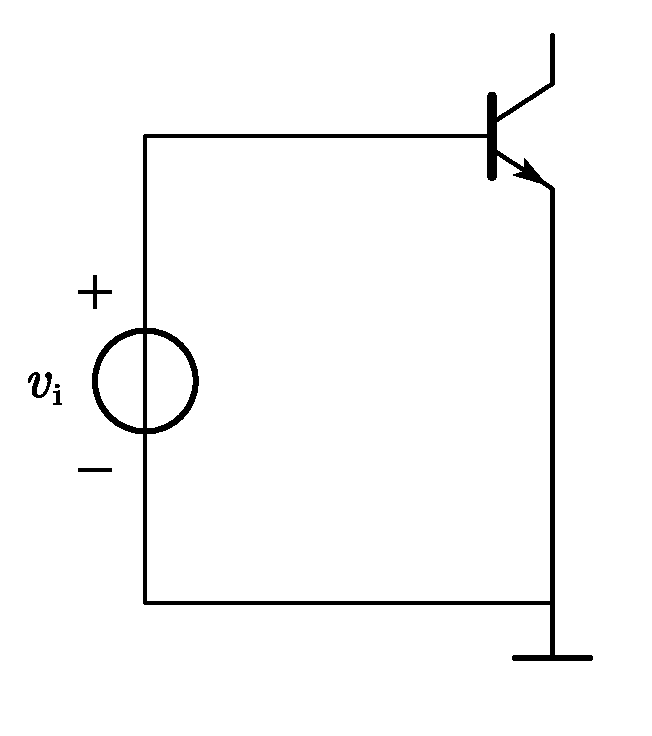
\includegraphics[width=0.35\linewidth]{pic/appendixApic/1.pdf}
    \caption{没有构建合理静态工作点的电路\label{1}}
\end{figure}

为了使BJT工作在放大区,需要在基极b和发射极e之间、集电极c和发射极e之间分别加上适当的直流电源$V_\mathrm{BB}$和$V_\mathrm{CC}$,使得发射结正偏、集电结反偏,如图\ref{2}所示。同时需要加入一个限流电阻$R_\mathrm{b}$避免be之间电压过大。

\begin{figure}[htb]
    \centering
        \subcaptionbox{静态工作点合理的电路\label{2}}
        {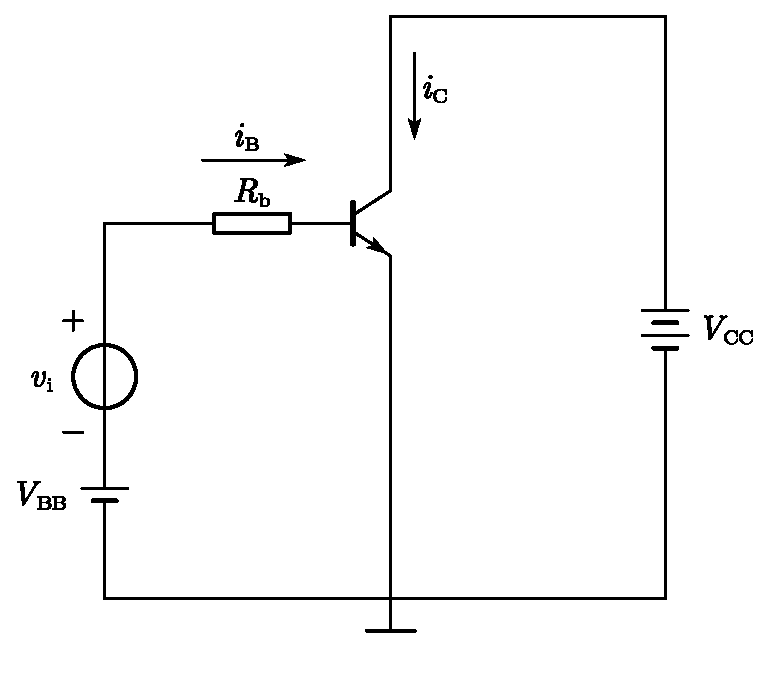
\includegraphics[width=0.35\linewidth]{pic/appendixApic/2.pdf}}\qquad
        \subcaptionbox{基本共射放大电路\label{3}}
        {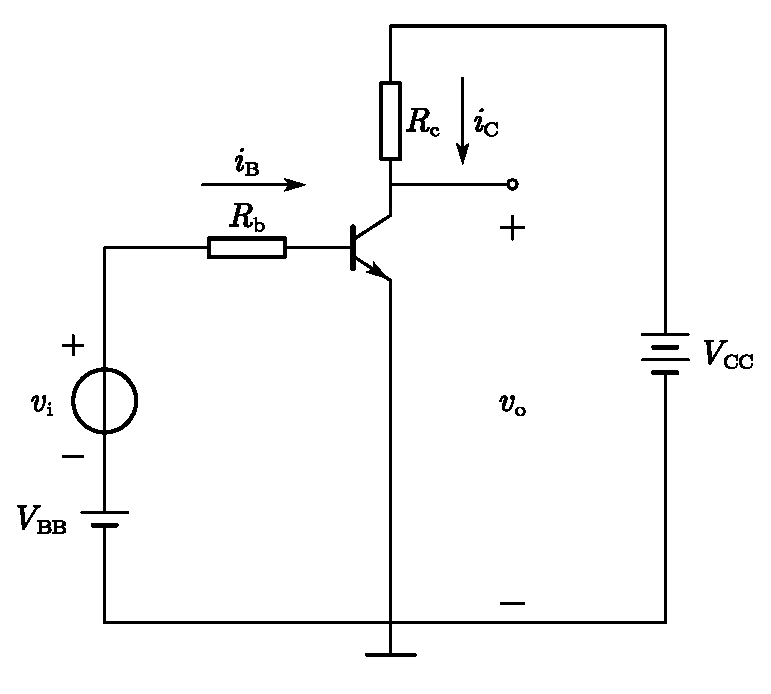
\includegraphics[width=0.35\linewidth]{pic/appendixApic/3.pdf}}
        \caption{基本共射放大电路的构成\label{静态工作点合理的电路}}
\end{figure}

通过构建合理的静态工作点,现在输入回路中$v_\mathrm{i}$引起$i_\mathrm{B}$的变化,会导致$i_\mathrm{C}$发生相应的变化。目前已经满足放大的所有要求了,但仍然存在一个问题——如何将$i_\mathrm{C}$的变化输出?最简单的思路是直接将负载接在$V_\mathrm{CC}$和BJT之间,但在实际操作中较为麻烦。另一种办法是在输出回路加上一个电阻$R_\mathrm{c}$,如图\ref{3}所示,将$i_\mathrm{C}$的变化转换为电压的变化,然后在集电极c和地之间输出。

\section{基本共射放大电路的改进}
通过以上的构造,就得到了基本共射放大电路,即第二章2.2.4小节中的图\ref{基本共射放大电路},现在希望优化其中的一些小细节。

电路存在的第一个问题是,电路中有两个电源$V_\mathrm{BB}$和$V_\mathrm{CC}$。实际上,只需要选择合适的$R_\mathrm{b}$和$R_\mathrm{c}$,就可以使得电源减少为一个,如图\ref{4}。稍作变化后可以得到图\ref{5}。
\begin{figure}[htb]
    \centering
        \subcaptionbox{变化前\label{4}}
        {\includegraphics[width=0.35\linewidth]{pic/appendixApic/4.pdf}}\qquad
        \subcaptionbox{变化后\label{5}}
        {\includegraphics[width=0.25\linewidth]{pic/appendixApic/5.pdf}}
        \caption{减少电源数量后的放大电路\label{减少电源数量后的放大电路}}
\end{figure}

但是在变化后,电路出现了新的问题——此时的信号源变成了“浮地”状态,这样会对信号的传输造成一定不良的影响。如果想要信号源接到地上,最简单的思路就是将信号源直接接在基极b和发射极e之间。但是,这样又会造成BJT无法工作在放大状态,类似于图\ref{1}。

因此,需要引入$R_\mathrm{b1}$,使得电路有合适的静态工作点(这一点通过将$v_\mathrm{i}$置零就可以看出),如图\ref{6}所示。这种电路称为\textbf{直接耦合}的放大电路。

\begin{figure}[htb]
    \centering
    \includegraphics[width=0.35\linewidth]{pic/appendixApic/6.pdf}
    \caption{直接耦合的放大电路\label{6}}
\end{figure}

当引入的电阻$R_\mathrm{b1}$后,交流信号会在$R_\mathrm{b1}$和$R_\mathrm{b2}$上有一定分压,导致放大倍数降低,而在输出端,由于静态工作点的存在,输出的信号为直流信号和交流信号二者的叠加,常常需要去除。

因此,可以在输入输出端各引入一个电容,使得输入信号可以直接加在三极管的输入端,且输出的信号没有直流分量,如图\ref{7}所示。这种电路称为\textbf{阻容耦合}的放大电路。

\begin{figure}[htb]
    \centering
    \includegraphics[width=0.35\linewidth]{pic/appendixApic/7.pdf}
    \caption{阻容耦合的放大电路\label{7}}
\end{figure}

\section{静态工作点的稳定}
静态工作点的稳定对于电路的放大至关重要,而温度往往是影响静态工作点的一个主要因素,温度的变化会导致静态工作点的漂移。

由BJT在不同温度下的工作特性曲线可以知道,温度上升,将会导致$i_\mathrm{C}$上升。如果能引入某个参数使得,在温度升高时使得$i_\mathrm{C}$下降,就能达到稳定静态工作点的目标。由于$i_\mathrm{C}$受到$v_{\mathrm{BE}}$控制,因此只需要让温度上升时$v_{\mathrm{BE}}$下降即可。

\begin{figure}[htb]
    \centering
        \subcaptionbox{引入负反馈后的电路\label{8}}
        {\includegraphics[width=0.35\linewidth]{pic/appendixApic/8.pdf}}\qquad
        \subcaptionbox{引入旁路电容后的电路\label{9}}
        {\includegraphics[width=0.35\linewidth]{pic/appendixApic/9.pdf}}
        \caption{静态工作点稳定的放大电路\label{静态工作点稳定的放大电路}}
\end{figure}

由图\ref{7}可以看出,静态情形下的射极电位已经是一个固定的值,无法随着$i_\mathrm{C}$的上升而改变。若此时在射极和接地点之间引入电阻$R_{\mathrm{e}}$,当$i_\mathrm{C}$上升时,射极电位$v_\mathrm{E}$随之上升,且变化量远大于基极电位$v_\mathrm{B}$变化。这样的一个负反馈机制就使得电路有一定的稳定性。

此外,为了使基极电位$v_\mathrm{B}$更稳定,可以在基极和接地点之间再引入一个电阻$R_{\mathrm{b2}}$,使得流经$R_{\mathrm{b2}}$的电流$i_{\mathrm{b2}}\gg i_{\mathrm{B}}$,则$v_\mathrm{B}$近似为两个电阻的分压,这样我们就得到了图\ref{8}。

由\ref{公式-共射放大电路增益}式,该电路的电压放大倍数为

\begin{equation}
    A_v=\frac{v_\mathrm{o}}{v_\mathrm{i}}=-\frac{\beta (R_\mathrm{c}\parallel R_\mathrm{L})}{r_\mathrm{be}+(1+\beta)R_\mathrm{e}}
\end{equation}

可以看出,$R_\mathrm{e}$导致电压的放大倍数降低了。为了使$R_\mathrm{e}$不出现在$A_v$的表达式中,可以在$R_\mathrm{e}$旁边并联一个\textbf{旁路电容}$C_\mathrm{e}$,此时在交流通路中$R_\mathrm{e}$就被短路了,如图\ref{9}所示。

这样,通过一步一步地分析问题、解决问题,就得到了一个性质较好的放大电路。
    %\input{appendixB.tex}
    
    \backmatter

    %\input{chap/afterword}
    \printbibliography[heading=bibintoc]
    
    \catcode`\,=13
    \newcommand{,}{,}
    \newpage
    
    %\indexprologue{这里列出本手册所涉及的名词.}
    %\printindex
\end{document} 